
%----------------------------------------------------------------------------------------
%	PACKAGES AND OTHER DOCUMENT CONFIGURATIONS
%----------------------------------------------------------------------------------------
\PassOptionsToPackage{table}{xcolor}
\documentclass[
12pt, % The default document font size, options: 10pt, 11pt, 12pt
english, % ngerman for German
onehalfspacing, % Single line spacing, alternatives: 
headsepline, % Uncomment to get a line under the header
oneside,
]{MastersDoctoralThesis} % The class file specifying the document structure
%\usepackage[table,xcdraw]{xcolor}
\usepackage[utf8]{inputenc} % Required for inputting international characters
\usepackage[T1]{fontenc} % Output font encoding for international characters
\usepackage{palatino} % Use the Palatino font by default
\usepackage[backend=bibtex,style=numeric,natbib=true]{biblatex} % Use the bibtex backend with the authoryear citation style (which resembles APA)
%\addbibresource{example.bib} % The filename of the bibliography
\setcounter{secnumdepth}{3}

\addbibresource{references.bib} % The filename of the bibliography
\usepackage[autostyle=true]{csquotes} % Required to generate language-dependent quotes in the bibliography
\usepackage{algorithm}% http://ctan.org/pkg/algorithms
\usepackage{algpseudocode}% http://ctan.org/pkg/algorithmicx
\usepackage{amsmath}
\usepackage{caption}
\usepackage{subcaption}


%----------------------------------------------------------------------------------------
%	MARGIN SETTINGS
%----------------------------------------------------------------------------------------

\geometry{
	paper=a4paper, % Change to letterpaper for US letter
	inner=2.5cm, % Inner margin
	outer=3.8cm, % Outer margin
	bindingoffset=.5cm, % Binding offset
	top=1.5cm, % Top margin
	bottom=1.5cm, % Bottom margin
	%showframe, % Uncomment to show how the type block is set on the page
}

%----------------------------------------------------------------------------------------
%	THESIS INFORMATION
%----------------------------------------------------------------------------------------

\thesistitle{Thesis Title} % Your thesis title, this is used in the title and abstract, print it elsewhere with \ttitle
\supervisor{Vasilis Samoladas} % Your supervisor's name, this is used in the title page, print it elsewhere with \supname
\degree{Electrical and Computer Engineer} % Your degree name, this is used in the title page and abstract, print it elsewhere with \degreename
\author{Stefanos Stathatos} % Your name, this is used in the title page and abstract, print it elsewhere with \authorname

\subject{} % Your subject area, this is not currently used anywhere in the template, print it elsewhere with \subjectname
\keywords{} % Keywords for your thesis, this is not currently used anywhere in the template, print it elsewhere with \keywordnames
\university{\href{http://www.tuc.gr}{Technical University of Crete}} % Your university's name and URL, this is used in the title page and abstract, print it elsewhere with \univname
\department{\href{http://http://www.ece.tuc.gr/index.php?id=4101}{School of Electrical and Computer Engineering}} % Your department's name and URL, this is used in the title page and abstract, print it elsewhere with \deptname
\group{} % Your research group's name and URL, this is used in the title page, print it elsewhere with \groupname
\faculty{\href{http://www.tuc.gr}{Technical University of Crete}} % Your faculty's name and URL, this is used in the title page and abstract, print it elsewhere with \facname

\AtBeginDocument{
\hypersetup{pdftitle=\ttitle} % Set the PDF's title to your title
\hypersetup{pdfauthor=\authorname} % Set the PDF's author to your name
\hypersetup{pdfkeywords=\keywordnames} % Set the PDF's keywords to your keywords
}

\begin{document}

%\frontmatter % Use roman page numbering style (i, ii, iii, iv...) for the pre-content pages

\pagestyle{plain} % Default to the plain heading style until the thesis style is called for the body content



%----------------------------------------------------------------------------------------
%	TITLE PAGE
%----------------------------------------------------------------------------------------

\begin{titlepage}
\begin{center}

\vspace*{.06\textheight}
{\scshape\LARGE \univname\par}\vspace{1.5cm} % University name
\textsc{\Large Thesis}\\[0.5cm] % Thesis type

\HRule \\[0.4cm] % Horizontal line
{\huge \bfseries \ttitle\par}\vspace{0.4cm} % Thesis title
\HRule \\[1.5cm] % Horizontal line
 
\emph{Author:}\\
{\authorname} % Author name - remove the \href bracket to remove the link
\vspace{20pt}

\emph{Committee:} \\
{Associate Professor} {\supname} (Supervisor)\\
{Associate Professor} Minos Garofalakis\\
{Associate Professor} Kostas Petrakis\\
\vspace{20pt}
\vfill

\large \textit{A thesis submitted in fulfillment of the requirements\\ for the degree of \degreename}\\[0.3cm] % University requirement text
\textit{in the}\\[0.4cm]
\deptname\\\univname\\[2cm] % Research group name and department name
 
\vfill

{\large \today}\\[4cm] % Date
%\includegraphics{Logo} % University/department logo - uncomment to place it
 
\vfill
\end{center}
\end{titlepage}


%----------------------------------------------------------------------------------------
%	ABSTRACT PAGE
%----------------------------------------------------------------------------------------

\begin{abstract}
\addchaptertocentry{\abstractname} % Add the abstract to the table of contents
The huge growth of Web in the last years has lead to the demand for specialized applications, which operate in different devices, are secure and guarantee the constant provision of services to the user, under any circumstances. The software development process can be delivered at the same time by multiple stakeholders, which are located in different areas of the world, studying and working on the same code. The model driven software development is a design technique which is based in model utilization and assists in the creation of software, which is extensible, reusable and comprehensible by different stakeholders. It contributes in the development of isolated modules with seperated responsibilities.\par 
	Another challenge of the time we are in, is the daily touch with large amounts of complex data, which one must constantly study in order to draw conclusions and make decisions. Due to the way the human brain processes information, using charts or graphs to visualize data is easier than studying spreadsheets or reports.  \par 
	In this thesis, we developed a data visualization framework, which follows the principles of model driven programming. The hierarchical data format is utilized for storing complex multidimensional datasets. The framework consists of modules which contain generic code and are configurable by other modules. The framework's functionality is expanded, either through the development of a new independent module or via the growth of an existing one. The framework presentation is implemented through the creation of a web application, which operates as a data visualization tool, for networks of users working on the same projects. The framework, as well as the application, are mainly developed in the javascript programming language.




\end{abstract}

%----------------------------------------------------------------------------------------
%	ACKNOWLEDGEMENTS
%----------------------------------------------------------------------------------------

\begin{acknowledgements}
\addchaptertocentry{\acknowledgementname} % Add the acknowledgements to the table of contents
The acknowledgments and the people to thank go here, don't forget to include your project advisor\ldots
\end{acknowledgements}

%----------------------------------------------------------------------------------------
%	LIST OF CONTENTS/FIGURES/TABLES PAGES
%----------------------------------------------------------------------------------------

\tableofcontents % Prints the main table of contents

\listoffigures % Prints the list of figures

\listoftables
%----------------------------------------------------------------------------------------
%	THESIS CONTENT - CHAPTERS
%----------------------------------------------------------------------------------------

\mainmatter % Begin numeric (1,2,3...) page numbering

\pagestyle{thesis} % Return the page headers back to the "thesis" style

% Introduction

\chapter{Introduction} % Main chapter title

\section{Overview}
The World Wide Web has been central to the development of the Information Age and is the primary tool billions of people use to interact on the Internet. The huge growth of Web in the last years has lead to the demand for specialized applications, which operate in different devices, are secure and guarantee the constant provision of services to the user, under any circumstances. The software development process can be delivered at the same time by multiple stakeholders, which are located in different areas of the world, studying and working on the same code. Meanwhile, the time-consuming stages of production necessitate the proper software design, with the purpose of minimizing the possibility of large design flaws or discovering them in early stages. \par 
	The model driven software development is a design technique which is based in model utilization and assists in the creation of software, which is extensible, reusable and comprehensible by different stakeholders. It contributes in the development of isolated modules with seperated responsibilities. Hence, this design approach is an ideal solution for creating carefully developed, well tested software, which can be upgraded at any moment. \par 
	Another challenge of the time we are in, is the daily touch with large amounts of complex data, which one must constantly study in order to draw conclusions and make decisions. Because of the way the human brain processes information, using charts or graphs to visualize data is easier than poring over spreadsheets or reports. Data visualization is the presentation of data in a pictorial or graphical format. It enables decision makers to see analytics presented visually, so they can grasp difficult concepts or identify new patterns. \par
	In this thesis, we developed a data visualization framework, which follows the principles of model driven programming. The hierarchical data format is utilized for storing complex multidimensional datasets. The framework implements a method to present visually the datasets to the users, which enables easy understanding, conclusion extraction and decision making. \par 
	The framework consists of modules which contain generic code and are configurable by other modules. The framework's functionality is expanded, either through the development of a new independent module or via the growth of an existing one. The model driven approach enables the system's adaptability based on the designer's requirements. \par 
	The framework presentation is implemented through the creation of a web application, which operates as a data visualization tool, for networks of users working on the same projects. The projects contain datasets, posts and plots, which are visible by all project members. The plots are used as a graphical representation of the datasets. \par
	Among other things, the user may interact with the datasets through the diagrams. We implemented a zoom functionality, which enables  switching between the detail levels of the visualized datasets. While the abstract representation of large datasets is possible, the display of small details is also available. The retrieval of sampled chunks of HDF files makes the zoom functionality efficient.   \par 
	The framework, as well as the application, are mainly developed in the javascript programming language. Especially the front end tier was developed exclusively in pure javascript, without the usage of a large framework. The front end follows the principles of the single page application design approach.


%I terastia anaptuksi tou exei odigisei stin anagki gia dimiourgia ekseidikeumenwn efarmogwn, oi opoies leitourgoun se polles diaforetikes suskeues, einai asfaleis kai egguontai tin sunexi paroxi upiresiwn sto xristi upo opoiesdipote sunthikes. I idia i anaptuksi efarmogwn pleon mporei na ginetai apo apo pollous stakeholders tautoxrona, oi opoioi vriskontai se diaforetika simeia tou kosmou kai meletoun k epemvainoun se koino kwdika. Parallila, ta xronovora stadia paragwgis kathistoun megali proteraiotita ton swsto sxediasmo tou logismikou, etsi wste na elaxistopoiithoun i na anakalufthoun sta prwta stadia, megala sxediastika flaws. \par
%	To model-driven software development einai mia sxediastiki texniki i opoia vasizetai stin anaptuksi montelwn, kai voithaei stin paragwgi logismikou to opoio einai epektasimo, reusable kai eukola katanoito apo diaforetikous stakeholders. Suneisferei stin dimiourgia modules kwdika isolated metaksu tous kai me ksexwrista responsibilities. Epomenws, to sugekrimeno sxediastiko approach einai idaniki lusi gia tin dimiourgia prosektika grammenou tested logismikou pou mporei ana pasa stigmi na anavathmistei. \par
%	Ena allo xaraktiristiko tis epoxis pou dianioume einai i kathimerini epafi me large amounts of complex data, ta opoia prepei kaneis na meletaei wste na vgazei sumperasmata kai na pairnei apofaseis. Because of the way the human brain processes information, using charts or graphs to visualize data is easier than poring over spreadsheets or reports. Data visualization is the presentation of data in a pictorial or graphical format. It enables decision makers to see analytics presented visually, so they can grasp difficult concepts or identify new patterns. \par
%
%	In this thesis, anaptusoume ena data visualization framework, to opoio akolouthei tis arxes tou montelostrafous programmatismou. Xrisimopoiei to hierachical data format, gia na apothikeusei complex multidimentional datasets. To framework ulopoiei mia methodo dataset visualization stous xristes, to opoio epitrepei tin eukoli katanoisi, eksagwgi sumperasmatwn kai decision making. \par 
%	Gia tin anaptuksi tou, dimiourgithikan modules ta opoia periexoun generic kwdika kai einai parametropoiisima apo alla modules. Auto exei ws apotelesma tin paragwgi reusable kai extensible modules ta opoia sundiazontai metaksu tous gia tin dimiourgia tou framework. I parousiasi tou framework ginetai mesw tis dimiourgias mias web efarmogis, i opoia leitourgei ws ena data visualization tool gia diktua apo users oi opoioi ergazontai se koina projects. To framework, opws kai i efarmogi, ulopoiithikan sto megalutero vathmo se javascript.
\section{Outline}
Chapter ~\ref{chapter2_bg} provides the necessary theoretical background used throughout this thesis, including model driven software development, data access object, access control list and RESTful web service. An overview of the related work and technologies used is presented in chapter ~\ref{chapter3_rw}. The proposed detailed framework architecture is described in chapter ~\ref{chapter4_d}. In chapter~\ref{chapter5_i} we discuss the framework and application implementation as well as the technologies we utilized. Next, we evaluate the framework performance in chapter~\ref{chapter6_pe}. Finally, the conclusion and future work are presented in chapter~\ref{chapter7_cf}. 
% Background

\chapter{Background} % Main chapter title

\label{chapter2_bg}
This chapter presents some background for the content of this thesis. We introduce theoretical concepts, such as model driven software development, data access object, access control list, HTTP protocol and RESTful web services.

\section{Models and Model Driven Software Development}
\label{mdsd}
Software development is a complex and difficult task that requires the investment of significant resources and carries a major risk of failure. According to its proponents, model-driven (MD) software development approaches are improving the way we build software. Model-driven approaches hypothetically increase developer productivity, decrease the cost (in time and money) of software construction, improve software reusability, and make software more maintainable. Likewise, model-driven techniques promise to contribute to the early detection of defects such as design flaws, omissions, and misunderstandings between clients and developers. \par
	If a model is a representation of a system, then in some sense, programming in any language involves some kind of model. Whether we explicitly create artifacts we call models—especially conceptual models—or whether we implicitly map between our internal mental models of the world and the systems we produce, we are nevertheless involved in a modeling process as we construct software. And so MD is more about raising the level of abstraction of our programming models rather than introducing models into the process in the first place. Models  help software engineers communicate more effectively with the many stakeholders who need to participate in the software development process. Improved communication leads to increased understanding, more reasonable expectations, and a better overall work product. Models also let programmers visualize the finished product without requiring its full construction first. By examining the model we can discover design flaws that are far less expensive to resolve up-front rather than after construction has begun (or worse, been completed).\par
	Model-driven software development~\cite{liddle2011model} is a software design approach for the development of software systems. It provides a set of guidelines for the structuring of specifications, which are expressed as models. Model-driven architecture (MDA) is a kind of domain engineering, and supports model-driven engineering of software systems.\par
	The three primary goals of MDA are portability, interoperability, and reusability, and the key abstraction for delivering on these goals is architectural separation of concerns. Architectural separation of concerns is a design principle for separating a computer program into distinct sections, such that each section addresses a separate concern. A concern is a set of information that affects the code of a computer program. When concerns are well-separated, individual sections can be reused, as well as developed and updated independently. Of special value is the ability to later improve or modify one section of code without having to know the details of other sections, and without having to make corresponding changes to those sections. In this way, architectural separation of concerns accomplishes the primary goals of MDA. Thus, developing generic, customizable, independent modules with seperated responsibilities implements the model driven software development approach.
  


\section{Data Access Object}
\label{dao}
In computer software, a data access object (DAO)~\cite{DAO} is an object that provides an abstract interface to some type of database or other persistence mechanism. By mapping application calls to the persistence layer, the DAO provides some specific data operations without exposing details of the database. This isolation supports the single responsibility principle. It separates what data access the application needs, in terms of domain-specific objects and data types (the public interface of the DAO), from how these needs can be satisfied with a specific DBMS or database schema. Because the interface exposed by the DAO to clients does not change when the underlying data source implementation changes, this pattern allows the DAO to adapt to different storage schemes without affecting its clients or business components. Essentially, the DAO acts as an adaptor between the component and the data source.\par 
	The advantage of using data access objects is the relatively simple and rigorous separation between two important parts of an application that can but should not know anything of each other, and which can be expected to evolve frequently and independently. Changing business logic can rely on the same DAO interface, while changes to persistence logic do not affect DAO clients as long as the interface remains correctly implemented. All details of storage are hidden from the rest of the application. Thus, possible changes to the persistence mechanism can be implemented by just modifying one DAO implementation while the rest of the application isn't affected. DAOs act as an intermediary between the application and the database. They move data back and forth between objects and database records.

\section{Access Control List}
\label{acl}
An Access Control List (ACL)~\cite{shirey2007internet} is a mechanism that implements access control for a system resource by enumerating the system 	entities that are permitted to access the resource and stating, either implicitly or explicitly, the access modes granted to each entity. A filesystem ACL is a data structure (usually a table) containing entries that specify individual user or group rights to specific system objects such as programs, processes, or files. \par
	In computing, permission is defined as the delegation of authority over a computer system. A permission allows a user to perform an action. Examples of various privileges include the ability to create a file in a directory, or to read or delete a file, access a device, or have read or write permission to a socket for communicating over the Internet. The permissions to perform certain operations are assigned to specific roles. Members or administrators (or other system users) are assigned particular roles, and through those role assignments acquire the computer permissions to perform particular computer-system functions.

\section{HTTP}
The Hypertext Transfer Protocol (HTTP)~\cite{fielding2006hypertext} is an application-level protocol for distributed, collaborative, hypermedia information systems. HTTP has been in use by the World-Wide Web global information initiative since 1990. HTTP functions as a request–response protocol in the client–server computing model. A web browser, for example, may be the client and an application running on a computer hosting a website, may be the server. The client submits an HTTP request message to the server. The server, which provides resources such as HTML files and other content or performs other functions on behalf of the client, returns a response message to the client. The response contains completion status information about the request and may also contain requested content in its message body. HTTP resources are identified and located on the network by Uniform Resource Locators (URL), using the Uniform Resource Identifiers (URI) schemes http and https. URI and hyperlinks in HTML documents form inter-linked hypertext documents.




\subsection{HTTP session}
An HTTP session is a sequence of network request-response transactions. An HTTP client initiates a request by establishing a Transmission Control Protocol (TCP) connection to a particular port on a server. An HTTP server listening on that port waits for a client's request message. Upon receiving the request, the server sends back a status line, such as "HTTP/1.1 200 OK", and a message of its own. The body of this message is typically the requested resource, although an error message or other information may also be returned.




\subsection{Request methods}
HTTP defines methods to indicate the desired action to be performed on the identified resource. What this resource represents, whether pre-existing data or data that is generated dynamically, depends on the implementation of the server. The most common methods which are used in this thesis are presented below.

\paragraph{GET}
The GET method requests a representation of the specified resource. Requests using GET should only retrieve data and should have no other effect. The W3C has published guidance principles on this distinction, saying, "Web application design should be informed by the above principles but also by the relevant limitations".

\paragraph{POST}
The POST method requests that the server accepts the entity enclosed in the request as a new subordinate of the web resource identified by the URI. The data POSTed might be, for example, an annotation for existing resources; a message for a bulletin board, newsgroup, mailing list, or comment thread; a block of data that is the result of submitting a web form to a data-handling process; or an item to add to a database.

\paragraph{PUT}
The PUT method requests that the enclosed entity be stored under the supplied URI. If the URI refers to an already existing resource, it is modified; if the URI does not point to an existing resource, then the server can create the resource with that URI.

\paragraph{DELETE}
The DELETE method deletes the specified resource.




\subsection{Status Codes}
In HTTP/1.0 and since, the first line of the HTTP response is called the status line and includes a numeric status code (such as "404") and a textual reason phrase (such as "Not Found"). The way the user agent handles the response primarily depends on the code and secondarily on the other response header fields. Custom status codes can be used since, if the user agent encounters a code it does not recognize, it can use the first digit of the code to determine the general class of the response. HTTP status code is primarily divided into five groups for better explanation of request and responses between client and server, and are presented below. 

\paragraph{1xx Informational responses}
An informational response indicates that the request was received and understood. It is issued on a provisional basis while request processing continues. It alerts the client to wait for a final response. The message consists only of the status line and optional header fields, and is terminated by an empty line.

\paragraph{2xx Success}
This class of status codes indicates the action requested by the client was received, understood, accepted, and processed successfully.

\paragraph{3xx Redirection}
This class of status code indicates the client must take additional action to complete the request. Many of these status codes are used in URL redirection.
A user agent may carry out the additional action with no user interaction only if the method used in the second request is GET or HEAD. A user agent may automatically redirect a request. A user agent should detect and intervene to prevent cyclical redirects.

\paragraph{4xx Client errors}
This class of status code is intended for situations in which the client seems to have errored. Except when responding to a HEAD request, the server should include an entity containing an explanation of the error situation, and whether it is a temporary or permanent condition. These status codes are applicable to any request method. User agents should display any included entity to the user.

\paragraph{5xx Server errors}
The server failed to fulfill an apparently valid request: response status codes beginning with the digit "5" indicate cases in which the server is aware that it has encountered an error or is otherwise incapable of performing the request. Except when responding to a HEAD request, the server should include an entity containing an explanation of the error situation, and indicate whether it is a temporary or permanent condition. Likewise, user agents should display any included entity to the user. These response codes are applicable to any request method.




\section{Representational State Transfer}
\label{rest}
Representational state transfer (REST)~\cite{w3c2004web} or RESTful web services is a way of providing interoperability between computer systems on the Internet. REST-compliant Web services allow requesting systems to access and manipulate textual representations of Web resources using a uniform and predefined set of stateless operations.  In a RESTful Web service, requests made to a resource's URI will elicit a response that may be in XML, HTML, JSON or some other defined format. The response may confirm that some alteration has been made to the stored resource, and it may provide hypertext links to other related resources or collections of resources.\par  		The term is intended to evoke an image of how a well-designed Web application behaves: it is a network of Web resources (a virtual state-machine) where the user progresses through the application by selecting links, such as /user/tom, and operations such as GET or DELETE (state transitions), resulting in the next resource (representing the next state of the application) being transferred to the user. There are six guiding constraints that define a RESTful system. These constraints restrict the ways that the server may process and respond to client requests so that, by operating within these constraints, the service gains desirable non-functional properties, such as performance, scalability, simplicity, modifiability, visibility, portability, and reliability. If a service violates any of the required constraints, it cannot be considered RESTful. The formal REST constraints are represented below.

\subsection{Client-server architecture}
The first constraints added to our hybrid style are those of the client-server architectural style. Separation of concerns is the principle behind the client-server constraints. By separating the user interface concerns from the data storage concerns, we improve the portability of the user interface across multiple platforms and improve scalability by simplifying the server components. Perhaps most significant to the Web, however, is that the separation allows the components to evolve independently, thus supporting the Internet-scale requirement of multiple organizational domains.

\paragraph{Statelessness}
The client–server communication is constrained by no client context being stored on the server between requests. Each request from any client contains all the information necessary to service the request, and session state is held in the client. The session state can be transferred by the server to another service such as a database to maintain a persistent state for a period and allow authentication. The client begins sending requests when it is ready to make the transition to a new state. While one or more requests are outstanding, the client is considered to be in transition. The representation of each application state contains links that may be used the next time the client chooses to initiate a new state-transition.

\paragraph{Cacheability}
As on the World Wide Web, clients and intermediaries can cache responses. Responses must therefore, implicitly or explicitly, define themselves as cacheable or not to prevent clients from reusing stale or inappropriate data in response to further requests. Well-managed caching partially or completely eliminates some client–server interactions, further improving scalability and performance.

\paragraph{Layered system}
A client cannot ordinarily tell whether it is connected directly to the end server, or to an intermediary along the way. Intermediary servers may improve system scalability by enabling load balancing and by providing shared caches. They may also enforce security policies.

\paragraph{Uniform interface}
The uniform interface constraint is fundamental to the design of any REST service. It simplifies and decouples the architecture, which enables each part to evolve independently.





\section{Application Programming Interface}
In computer programming, an Application Programming Interface (API) is a set of subroutine definitions, protocols, and tools for building application software. In general terms, it is a set of clearly defined methods of communication between various software components. A good API makes it easier to develop a computer program by providing all the building blocks, which are then put together by the programmer. An API may be for a web-based system, operating system, database system, computer hardware or software library. An API specification can take many forms, but often includes specifications for routines, data structures, object classes, variables or remote calls. API uses are listed below.

\paragraph{Libraries and Frameworks}
An API is usually related to a software library. The API describes and prescribes the expected behavior (a specification) while the library is an actual implementation of this set of rules. A single API can have multiple implementations (or none, being abstract) in the form of different libraries that share the same programming interface. The separation of the API from its implementation can allow programs written in one language to use a library written in another. 

\paragraph{Operating systems}
An API can specify the interface between an application and the operating system. POSIX, for example, specifies a set of common APIs that aim to enable an application written for a POSIX conformant operating system to be compiled for another POSIX conformant operating system.

\paragraph{Remote APIs}
Remote APIs allow developers to manipulate remote resources through protocols, specific standards for communication that allow different technologies to work together, regardless of language or platform.


\paragraph{WEB APIs}
Web APIs are the defined interfaces through which interactions happen between an enterprise and applications that use its assets. An API approach is an architectural approach that revolves around providing programmable interfaces to a set of services to different applications serving different types of consumers.When used in the context of web development, an API is typically defined as a set of Hypertext Transfer Protocol (HTTP) request messages, along with a definition of the structure of response messages, which is usually in an Extensible Markup Language (XML) or JavaScript Object Notation (JSON) format.

\section{Three-tier Architecture}
\label{3tierarch}
\begin{figure}
	\centerline{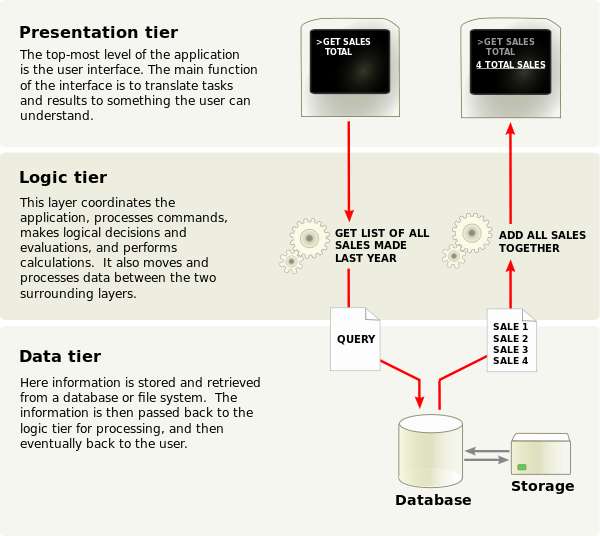
\includegraphics[scale=0.5]{3tier.png}}
	\caption{Three-tier Architecture}
	\label{3tier}
\end{figure}

Three-tier architecture~\cite{ramirez2000three} is a client–server software architecture pattern in which the user interface (presentation), functional process logic ("business rules"), computer data storage and data access are developed and maintained as independent modules, most often on separate platforms. Apart from the usual advantages of modular software with well-defined interfaces, the three-tier architecture is intended to allow any of the three tiers to be upgraded or replaced independently in response to changes in requirements or technology. An image of a three-tier architecture can be seen in figure~\ref{3tier}. The three layers are presented below.

\paragraph{Presentation tier}
This is the topmost level of the application. The presentation tier displays information related to such services as browsing merchandise, purchasing and shopping cart contents. It communicates with other tiers by which it puts out the results to the browser/client tier and all other tiers in the network. In simple terms, it is a layer which users can access directly (such as a web page, or an operating system's GUI).

\paragraph{Logic tier}
The logical tier is pulled out from the presentation tier and, as its own layer, it controls an application’s functionality by performing detailed processing.

\paragraph{Data tier}
The data tier includes the data persistence mechanisms (database servers, file shares, etc.) and the data access layer that encapsulates the persistence mechanisms and exposes the data. The data access layer should provide an API to the application tier that exposes methods of managing the stored data without exposing or creating dependencies on the data storage mechanisms. Avoiding dependencies on the storage mechanisms allows for updates or changes without the application tier clients being affected by or even aware of the change.




\section{Single Page Application}
\label{spa}
\begin{figure}
	\centerline{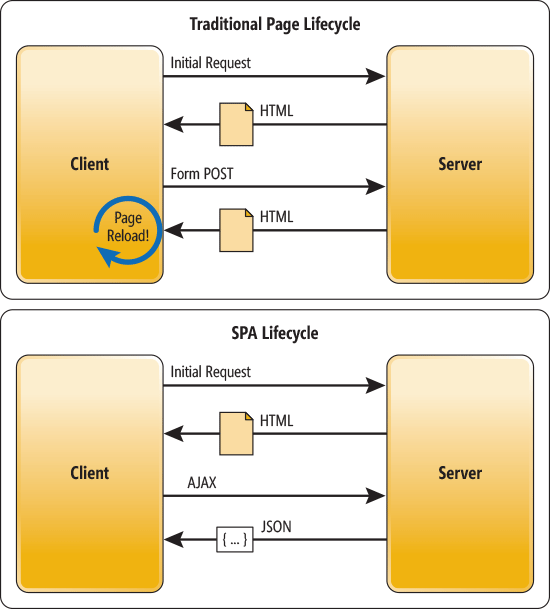
\includegraphics[scale=0.4]{spa.png}}
	\caption{Traditional page lifecycle vs Single Page Application Lifecycle}
	\label{spa}
\end{figure}
A single-page application (SPA)~\cite{mikowski2013single} is a web application or web site that fits on a single web page with the goal of providing a user experience similar to that of a desktop application. In a SPA, either all necessary code – HTML, JavaScript, and CSS – is retrieved with a single page load, or the appropriate resources are dynamically loaded and added to the page as necessary, usually in response to user actions. The page does not reload at any point in the process, nor does control transfer to another page, although the location hash or the HTML5 History API can be used to provide the perception and navigability of separate logical pages in the application. Interaction with the single page application often involves dynamic communication with the web server behind the scenes.\par
	There are various techniques available that enable the browser to retain a single page even when the application requires server communication. The most prominent technique currently being used is Ajax. Ajax is a set of Web development techniques using many Web technologies on the client side to create asynchronous Web applications. With Ajax, Web applications can send data to and retrieve from a server asynchronously (in the background) without interfering with the display and behavior of the existing page. By decoupling the data interchange layer from the presentation layer, Ajax allows for Web pages, and by extension Web applications, to change content dynamically without the need to reload the entire page. The difference between the traditional page and the SPA lifecycle can be seen in figure~\ref{spa}. In practice, modern implementations commonly substitute JSON for XML due to the advantages of being native to JavaScript.



\section{Hierarchical Data Format}
\label{hdf}
\begin{figure}
	\centerline{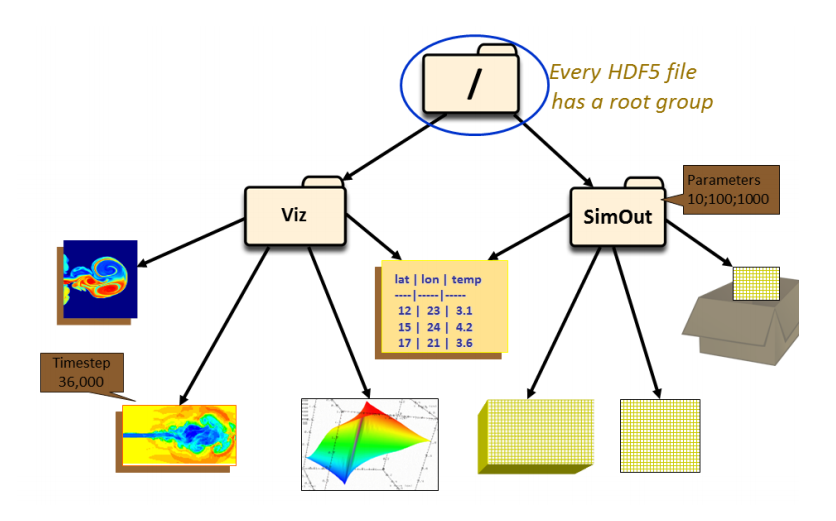
\includegraphics[scale=0.4]{hdf.png}}
	\caption{The contents of an HDF file}
	\label{hdf}
\end{figure}
\begin{figure}
	\centerline{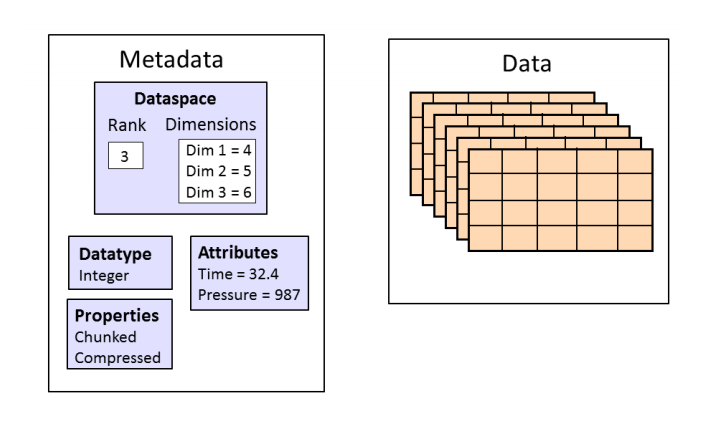
\includegraphics[scale=0.5]{dset.png}}
	\caption{The general structure of a dataset}
	\label{dset}
\end{figure}
Hierarchical Data Format (HDF))~\cite{hdf2014hierarchical} is a set of file formats (HDF4, HDF5) designed to store and organize large amounts of data. Many HDF adopters have very large datasets, very fast access requirements, or very complex datasets. Others turn to HDF because it allows them to easily share data across a wide variety of computational platforms using applications written in different programming languages.\par
	HDF allows hierarchical data objects to be expressed in a very natural manner, in contrast to the tables of a relational database.  Whereas relational databases support tables, HDF supports n-dimensional datasets and each element in the dataset may itself be a complex object. Relational databases offer excellent support for queries based on field matching, but are not well-suited for sequentially processing all records in the database or for subsetting the data based on coordinate-style lookup. The contents of an HDF file can be seen in figure~\ref{hdf}.\par
	HDF5 consists of a File Format for storing HDF5 data, a Data Model for logically organizing and accessing HDF5 data from an application, and the Software (libraries, language interfaces, and tools) for working with this format. The data model is described below.
\subsection{Data Model}
The HDF Data Model, also known as the HDF5 Abstract (or Logical) Data Model consists of the building blocks for data organization and specification in HDF5. An HDF5 file (an object in itself) can be thought of as a container (or group) that holds a variety of heterogeneous data objects (or datasets). The datasets can be most anything: images, tables, graphs, or even documents, such as PDF or Excel. The two primary objects in the HDF5 Data Model are described below.

\paragraph{Groups}
HDF5 groups (and links) organize data objects. Every HDF5 file contains a root group that can contain other groups or be linked to objects in other files. Working with groups and group members is similar in many ways to working with directories and files in UNIX. As with UNIX directories and files, objects in an HDF5 file are often described by giving their full (or absolute) path names.

\paragraph{Datasets}
HDF5 datasets organize and contain the “raw” data values. A dataset consists of metadata that describes the data, in addition to the data itself. Datatypes, dataspaces, properties and (optional) attributes are HDF5 objects that describe a dataset. The datatype describes the individual data elements. The general structure of a dataset can be seen in figure~\ref{dset}.













% Related Work

\chapter{Related Work and Technologies Used} % Main chapter title

\label{chapter3_rw}
This chapter contains the related work and the technologies used throughout this thesis. Initially, technologies that make use of functionalities similar with the content of our framework, are described. Following, we emphasize on the technologies we used throughout the development of our system.

\section{Related Work}

\subsection{Plotly}
Plotly is a popular public data visualization cloud service provider. Plotly provides community, professional and enterprise data storage, visualization and analytics services to the user.  Excel, CSV and XML data formats are used to upload the data to its cloud servers.  It also offers online graphing, analytics, and statistics tools for individuals and collaboration, as well as scientific graphing libraries for Python, R, MATLAB, Perl, Julia, Arduino, and REST. Although Plotly provides a large set of functionalities, it does not offer a way to visualize large multidimensional datasets.

\subsection{Loopback}
Loopback is a highly-extensible, open-source Node.js framework which assimilates the best practices of model driven software development. Loopback simplifies and speeds up REST API development. It consists of a library of Node.js modules for connecting web and mobile apps to data sources such as databases and REST APIs, a command line tool, and client-SDKs. A loopback application has three components: models that represent business data and behavior, data sources and connectors, and mobile clients. An application interacts with data sources through the loopback model API, available locally within Node, remotely over REST, and via native client APIs for iOS, Android, and HTML5. Using the API, apps can query databases, store data, upload files, send emails, create push notifications, register users, and perform other actions provided by data sources.
	Loopback is implemented with many of the technologies we use in this thesis. It uses MDSD as a general practice, data access objects for the communication between database and the server, access control list for  authorization and is written in Node.js.

\section{Technologies Used}

\subsection{HTML5}
HTML5~\cite{pilgrim2010html5} is a markup language used for structuring and presenting content on the World Wide Web. It is the fifth and current major version of the HTML standard.\par
It was published in October 2014 by the World Wide Web Consortium (W3C) to improve the language with support for the latest multimedia, while keeping it both easily readable by humans and consistently understood by computers and devices such as web browsers, parsers, etc. HTML5 is intended to subsume not only HTML 4, but also XHTML 1 and DOM Level 2 HTML.\par
HTML5 includes detailed processing models to encourage more interoperable implementations; it extends, improves and rationalizes the markup available for documents, and introduces markup and application programming interfaces (APIs) for complex web applications. For the same reasons, HTML5 is also a candidate for cross-platform mobile applications, because it includes features designed with low-powered devices in mind.

\subsection{CSS3}
Cascading Style Sheets (CSS) is a style sheet language used for describing the presentation of a document written in a markup language. Although most often used to set the visual style of web pages and user interfaces written in HTML and XHTML, the language can be applied to any XML document, including plain XML, SVG and XUL, and is applicable to rendering in speech, or on other media. Along with HTML and JavaScript, CSS is a cornerstone technology used by most websites to create visually engaging webpages, user interfaces for web applications, and user interfaces for many mobile applications.\par
CSS is designed primarily to enable the separation of presentation and content, including aspects such as the layout, colors, and fonts. This separation can improve content accessibility, provide more flexibility and control in the specification of presentation characteristics, enable multiple HTML pages to share formatting by specifying the relevant CSS in a separate .css file, and reduce complexity and repetition in the structural content. CSS3~\cite{mcfarland2012css3} is the latest version of CSS and is used in this thesis.


\subsection{Javascript}
JavaScript (JS)~\cite{crockford2008javascript} is a high-level, dynamic, weakly typed, object-based, multi-paradigm, and interpreted programming language. Alongside HTML and CSS, JavaScript is one of the three core technologies of World Wide Web content production. It is used to make webpages interactive and provide online programs, including video games. As a multi-paradigm language, JavaScript supports event-driven, functional, and imperative (including object-oriented and prototype-based) programming styles. Initially only implemented client-side in web browsers, JavaScript engines are now embedded in many other types of host software, including server-side in web servers and databases. The most famous server-side Javascript implementation is Node.js.

\subsubsection{Node.js}
\begin{figure}
	\centerline{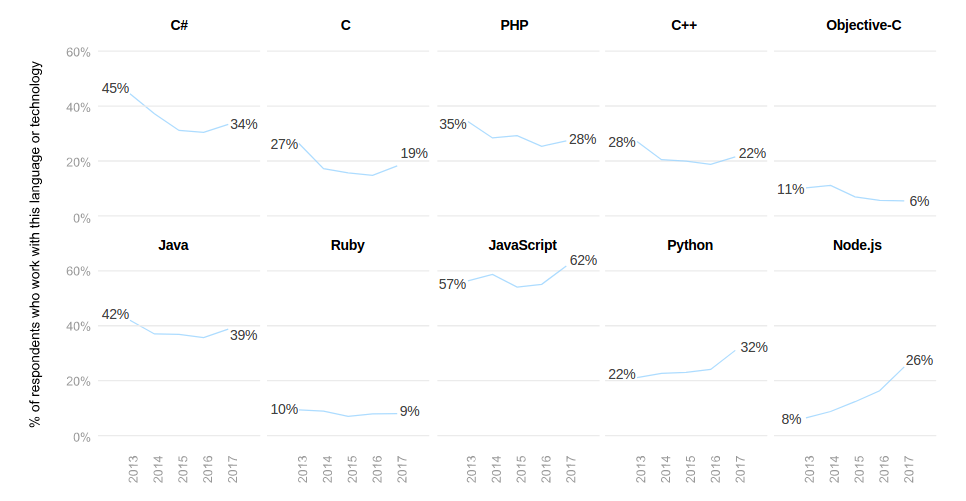
\includegraphics[scale=0.5]{survey17.png}}
	\caption{Developers survey for Stack Overflow website in 2017.}
	\label{survey17}
\end{figure}
Node.js~\cite{tilkov2010node} is an open-source, cross-platform JavaScript run-time environment for executing JavaScript code server-side. Node.js provides an event-driven architecture and a non-blocking I/O API designed to optimize application's throughput and scalability for real-time Web applications. It uses Google V8 JavaScript engine to execute code, and a large percentage of the basic modules are written in JavaScript. Node.js contains a built-in library to allow applications to act as a stand-alone Web server. The increasing popularity of Node.js in the last years can be seen in figure~\ref{survey17}.

\subsubsection{JSON}
\label{json}
In computing, JavaScript Object Notation or JSON~\cite{crockford2006application}, is an open-standard file format that uses human-readable text to transmit data objects consisting of attribute–value pairs and array data types (or any other serializable value). It is a very common data format used for asynchronous browser/server communication, including as a replacement for XML in some AJAX-style systems.
JSON is a language-independent data format. It was derived from JavaScript, but as of 2017 many programming languages include code to generate and parse JSON-format data. The official Internet media type for JSON is application/json. JSON filenames use the extension .json. JSON's basic data types are described below. \par
\paragraph{Number} A signed decimal number that may contain a fractional part and may use exponential E notation, but cannot include non-numbers like NaN. The format makes no distinction between integer and floating-point. JavaScript uses a double-precision floating-point format for all its numeric values, but other languages implementing JSON may encode numbers differently.
\paragraph{String} A string is a sequence of zero or more Unicode characters. Strings are delimited with double-quotation marks and support a backslash escaping syntax.
\paragraph{Boolean} Either of the values true or false.
\paragraph{Array} An ordered list of zero or more values, each of which may be of any type. Arrays use square bracket notation with elements being comma-separated.
\paragraph{Object} An unordered collection of name/value pairs where the names (also called keys) are strings. Since objects are intended to represent associative arrays, it is recommended, though not required, that each key is unique within an object. Objects are delimited with curly brackets and use commas to separate each pair, while within each pair the colon ':' character separates the key or name from its value.
\paragraph{null} An empty value, using the word null.

\subsubsection{Ajax}
\label{ajax}
\begin{figure}
	\centerline{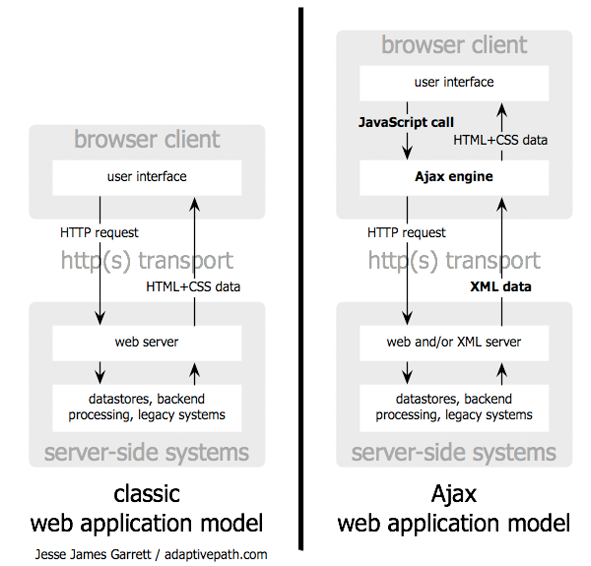
\includegraphics[scale=0.7]{ajax.png}}
	\caption{The traditional model for web applications (left) compared to the Ajax model (right)}
	\label{ajaxPNG}
\end{figure}
Ajax (short for "asynchronous JavaScript and XML")~\cite{garrett2005ajax} is a set of Web development techniques using many Web technologies on the client side to create asynchronous Web applications. With Ajax, Web applications can send data to and retrieve from a server asynchronously (in the background) without interfering with the display and behavior of the existing page. By decoupling the data interchange layer from the presentation layer, Ajax allows for Web pages, and by extension Web applications, to change content dynamically without the need to reload the entire page. In practice, modern implementations commonly substitute JSON for XML due to the advantages of being native to JavaScript.\par
Ajax is not a single technology, but rather a group of technologies. HTML and CSS can be used in combination to mark up and style information. The DOM is accessed with JavaScript to dynamically display – and allow the user to interact with – the information presented. JavaScript and the XMLHttpRequest object provide a method for exchanging data asynchronously between browser and server to avoid full page reloads.\par 
The term Ajax has come to represent a broad group of Web technologies that can be used to implement a Web application that communicates with a server in the background, without interfering with the current state of the page, such as HTML, CSS, DOM, XMLHttpRequest etc. The conventional model for a Web Application versus an application using Ajax can be seen in figure~\ref{ajaxPNG}.

\subsubsection{Node Package Manager}
Npm~\cite{schlueternode} is a package manager for the JavaScript programming language. It is the default package manager for the JavaScript runtime environment Node.js. It consists of a command line client, also called npm, and an online database of public packages called the npm registry. The registry is accessed via the client, and the available packages can be browsed and searched via the npm website. Npm is included as a recommended feature in Node.js installer. Npm consists of a command line client that interacts with a remote registry. It allows users to consume and distribute JavaScript modules that are available on the registry. Packages on the registry are in CommonJS format and include a metadata file in JSON format.

\subsection{NoSQL Database}
A NoSQL (originally referring to "non SQL" or "non-relational") database provides a mechanism for storage and retrieval of data that is modeled in means other than the tabular relations used in relational databases. NoSQL databases are increasingly used in big data and real-time web applications. Motivations for this approach include: simplicity of design, simpler "horizontal" scaling to clusters of machines (which is a problem for relational databases), and finer control over availability. The data structures used by NoSQL databases (e.g. key-value, wide column, graph, or document) are different from those used by default in relational databases, making some operations faster in NoSQL. The particular suitability of a given NoSQL database depends on the problem it must solve. Sometimes the data structures used by NoSQL databases are also viewed as "more flexible" than relational database tables.

\subsubsection{MongoDB}
MongoDB is a free and open-source cross-platform document-oriented database program. Instead of using tables and rows as in relational databases, MongoDB is built on an architecture of collections and documents, meaning fields can vary from document to document and data structure can be changed over time. Documents comprise sets of key-value pairs and are the basic unit of data in MongoDB. Collections contain sets of documents and function as the equivalent of relational database tables. \par 
	Like other NoSQL databases, MongoDB supports dynamic schema design, allowing the documents in a collection to have different fields and structures. The database uses a document storage and data interchange format called BSON, which provides a binary representation of JSON-like documents.



%System Design

\chapter{Design} % Main chapter title

This chapter provides a detailed description of the designed system. In section ~\ref{gfd}, the general framework design diagram is presented, along with a simplifying description of each module the diagram contains. 


\section{Framework Design}
\label{gfd}
\begin{figure}
	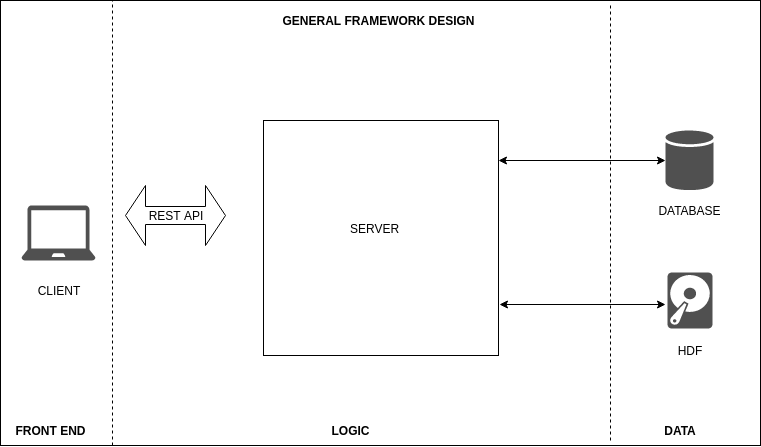
\includegraphics[scale=0.5]{framework.png}
	\caption{General Framework Design}
	\label{framework}
\end{figure}
In figure~\ref{framework} a general framework design diagram is presented. The system architecture is divided in three parts: front-end/presentation tier, logic tier and data tier, as described in chapter~\ref{3tierarch}. The data tier contains the database where all model data is stored, and the filesystem in which all uploaded datasets are saved in hdf form. The logic tier contains all the modules necessary for ensuring the framework functionality, such as crud operations, database access, authentication, authorization etc. The communication between logic and presentation tier is established over a rest api service. In the presentation tier, the user may interact with the server by sending requests and retrieve JSON data as responses. Before we continue in further details about the core system modules, next we describe the basic concepts of the application we created on top of our framework, in order to better demonstrate its capabilities.

\section{Application description}
The application makes use of the infrastructure which the framework implements, aiming to present an example of a real use case. Its purpose is to create user networks, which work on common projects with their data. These data could be text or multi-dimentional datasets. The application implements data visualization, with purpose the better understanding and conclusion extraction from the arithmetic datasets. The users may upload their datasets (in hdf form), in order to become visible from all the project users, while at the same time they may create plots based on them. In this chapter we describe the general design of the framework, but we provide some application design details when necessary. The detailed application implementation and functionality is presented in the next chapter.

\section{Generic Framework Modules}
In this section the framework modules used in this thesis are presented in detail. Diagrams are shown in some of these subsections for better understanding of the framework design. The modules are divided in three big categories: nosql access, main server and user interface. All modules and submodules are developed in a generic way, are highly customizable, extendible and reusable. This gives us the opportunity to often refer to these modules as models, as described in chapter~\ref{mdsd}. The level of abstraction may change, but the main characteristics of model driven software development are common in the framework implementation. Also, all modules are isolated and expose only the methods that must be used in the rest of the framework.


\subsection{Nosql access}
\label{nosql}
\begin{figure}
	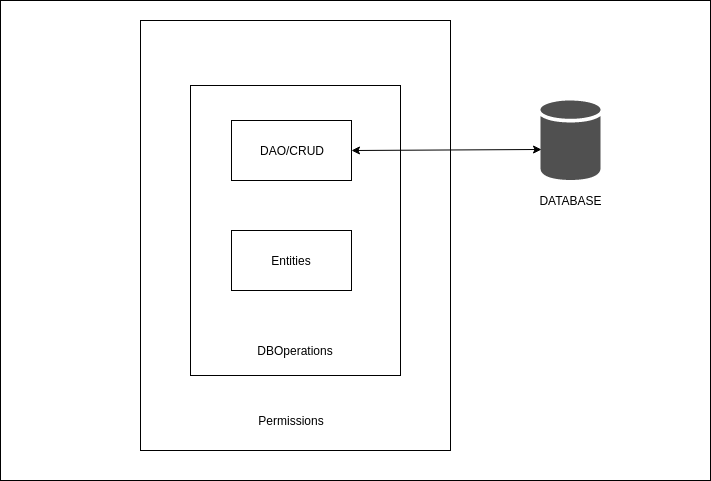
\includegraphics[scale=0.5]{nosqlaccess.png}
	\caption{NoSQL access module structure}
	\label{nosqlaccess}
\end{figure}
The nosql access module is a very important component of the framework. It is responsible for a big part of the system's functionality, such as schema creation, CRUD operations generation, communication between server and database etc. As a result of its importance, this module is used as a dependency in many other models of the framework. This model is developed in such a way, so its functionality is isolated from the rest of the framework. Aside from the fact that this practice applies to the model-driven approach, it is generally a clean way for developing frameworks. The structure of the module can be seen in figure ~\ref{nosqlaccess}. Nosql access module consists of many submodules and each of those is presented separately below. 

\subsubsection{Entities}
\label{entities}
An entity is a representation of a database resource. The creation of an entity through our framework, corresponds to the creation of a collection in our database. Likewise, the creation of an instance of an entity, corresponds to the creation of a document inside a collection in our database. In this way it becomes very easy to make changes to the database, without having direct access to it, which is crucial for our framework.\par
	In the entities module, we define the entities we are going to use in the framework. More specific, we define the structure of the entities we use, their fields, their fields type, as well as the fields restrictions. For example, we can define if a field must be unique in relation with the rest of the instances in the same collection of the database. The definition of the entities is written in JSON form, so it becomes really easy to change or add more entities in the database. So, this module obtains the property of extensibility, which is really important for the model-driven architecture we created. \par 
	For the purpose of the application demo, we defined a list of entities with specific fields, field types and restrictions. A visualization of this list is shown in figure MPLAAAAA. An analysis of each of the entities can be seen below.\par
	
	 
\paragraph{Users}
In order to use the application, a user is obligated to create a new user account. The necessary properties to create a new account are username, full name, password and email. Username and email must have unique values in relation with all other user instances. The entity Users contains all necessary fields to save the above information, in the addition of a unique id.
\paragraph{Projects}
A basic concept of the application is the project entity. The application users may create new projects, in which multiple users may participate. The content of a project is visible for all users that participate in it. The required fields for the creation of a project instance are name, date and description. The project entity uses the concept of ACL, as described in chapter~\ref{acl}. Thus, project entity contains information about which users can or cannot, use a CRUD operation for the specific instance of the project entity. This way, the fields that contain this information reference an instance of a user entity.
\paragraph{Datasets}
Another usefull entity of the application is Datasets. The application users may create their own datasets inside a project they participate. In this entity are saved the metadata of an hdf file which was uploaded on the application. The fields of this entity are the dataset name, date, a reference to the user instance who creates the entity, and the hdf filename. Also, a project instance reference,in which the dataset is in, is saved. Last, just as in project entity, information is retained about the access control list of the dataset.
\paragraph{Posts}
An application user may create a new post inside a project. The required fields for the creation of a post entity are title, description, date, a dataset instance reference and a project instance reference. Also, acl information  is saved in the post entity instance. The user may create a post in response of another post. In that case, information is retained about the post instance in reference.
\paragraph{Plots}
A user may add plots inside his posts. The required fields for the creation of a post entity are title, description, the path inside the hdf file in which the array used for the plot is saved, and the post instance reference. Also, the plot entity retains information about its metadata, such as plot type and the dimention values used in the plot.

\subsubsection{Data Access Object/ CRUD}
\label{daocrud}
As described in chapter~\ref{dao}, DAO provides some specific data operations without exposing details of the database which are not needed. In our case, the dao model ensures that it is the only module with access in the database, and exposes only the information and CRUD functions which are vital for the rest of the framework. The dao module is developed in a generic way and it is customizable by the entities module. Thus, for each of our entities, we generate CRUD operations for interaction between the specific database model and the framework. The CRUD methods used in the dao module are described in detail below.

\paragraph{createItem}
The method createItem is responsible for the creation of new instances of an entity. It receives an object as an argument, it converts it in model instance form and then saves it. If an error occures, it returns a new Error object. Based in the single responsibility principle, the method does not control the kind of data that are about to be saved.
\paragraph{readItems}
The method readItems is used to read data from the database. It receives a query object as an input. The result, successfull or not, is returned as an array object. If an error occures, it returns a new Error object.
\paragraph{updateItem}
The method updateItem is responsible for updating an existing object in the database. To achieve that, it receives as arguments a query object and an object with the new property values. If found, the object is replaced and returned. If an error occures, it returns a new Error object.
\paragraph{deleteItem}
The method deleteItem is used to delete an existing document from the database. It receives a query object as an input, and if the document is found, the method deletes it from the database. If an error occures, it returns a new Error object.

\subsubsection{DbOperations}
As mentioned in the section~\ref{daocrud}, the DAO module is responsible for interacting with the database. The model methods are interacting with the database, perform direct changes and may return a result where applicable. But is there a way to guarantee the integrity of our operations in live data? Throughout our study, we determined that all functions must be wrapped in functions responsible for the verification and validation of the requested data mutation. So in essense, we provide a single sandboxed environment securing the database from malicious adversaries, as well as potential internal missuse. \par 
	The DBOperations model was developed for this purpose. It receives as an argument the entities and the dao models. The DBOperations model returns a group of functions which control the data they receive as an input and then call the corresponding dao model methods. \par 
	The verification of the data is essential for the CRUD operations. In our case we primarily check if all the required properties and references are contained in the input object. Then, we verify that the references values are valid id's of the corresponding entities instance. In order to achieve that, the necessary read operations in the database are made.
	
\subsubsection{Permissions}
In chapter~\ref{entities}, we described that most of the entities contain some fields that are responsible for the accesss control list. To be able to alter these fields in relation with who can access or not a resource, we developed a module specialized for this task. This module contains some functions which implement the acl functionality. The dependencies of permissions model are entities and DBOperations models. \par 
	The Permissions modules defines all the roles the framework uses. At anytime we can add or remove a role, therefore the model-driven design approach is implemented. This model is also responsible for the verification of the changes that it is about to make. The module exposes only the desired methods, so that any unwanted functionality is isolated. The generic methods we developed are described below. 

\paragraph{addUserRole}
This method adds a specific role to a user for the given resource. It receives four arguments as an input, the user id, the object id, the role and the model name. All arguments are verified before proceeding with the entity instance update.
\paragraph{removeUserRole}
RemoveUserRole is a method that does the opposite of the addUserRole. It removes from a user a certain role of a resource. It also receives the same arguments as an input. All arguments are verified before proceeding with the entity instance update.
\paragraph{isAllowed}
This method is the core of the acl logic. Its purpose is to check if  a user has the permission to perform a crud operation in a resource instance. To accomplish that, this method checks if a user id is contained in the model instance of the resource id which is given as an input. If its not found, the same check is performed in the parent model instance, if it exists. \par 
	The reason behind this extra check, is that the parent model instance, may have been given a default order which applies for every kid model instance. This operation has the advantage, that we reduce many database operations, since we dont have to check the access permission of -usually many- users, each time we create a new kid model instance. On the contrary, we set a general rule which applies in all cases, unless it is overriden by another permission access. \par
	An example of this functionality is the creation of a post inside a project. One way to apply permission access, is to add all user id's which have read permission for the post, inside its instance. It is preferable though, to set a general rule inside the project which states that, all users who have read access to this project, have also access to its posts.

\paragraph{isAllowedCreate}
isAllowedCreate had the same functionality as isAllowed method, but it focuses exclusively on create operation, which has slightly different functionality than the rest of them.

\subsection{Main server}
\begin{figure}
	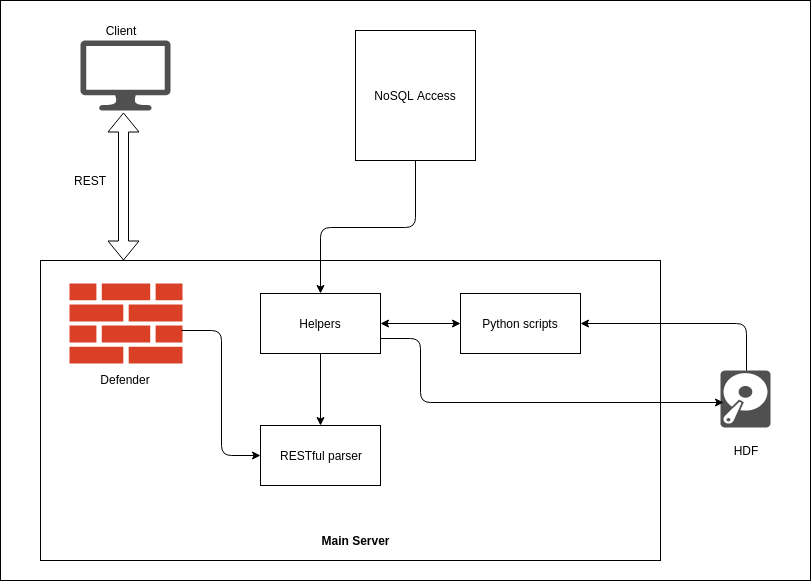
\includegraphics[scale=0.5]{mainserver.png}
	\caption{Main server module structure}
	\label{mainserver}
\end{figure}
In this section we describe the core framework's component.  The structure of this module can be seen in figure ~\ref{mainserver}. To achieve that, we present all the submodules that are used in this model, and combined together are creating its complete functionality. Thus, apart from routes module which is responsible for receiving requests and sending responds to the client, it is also described the helpers module, which is containing a list of functions necessary for this model. Also, in this chapter we present a python bridge model, which is used for the utilization of the hierarchical data format, as well as our error handling model, our session setup module and the defenders module. Next we describe each of these modules.

\subsubsection{Helpers}
\label{helpers}
In chapter~\ref{nosql} we defined a list of methods which are responsible for the communication with the database. In order to implement the framework's functionality though, it is necessary to combine these methods into a higher level module. The helpers model is developed for this reason and receives as an argument the nosql access module. Also, this module has a dependency on a list of python files, which are vital for the retrieval of saved hdf files (hdf explained in chapter~\ref{hdf}). The returned result of this module's methods is the one that is sent to the client. \par
	Next we are going to present some of these functions. Most of them are developed in conjunction with the application demo, but the module is extendible for any usage. We will skip the functions which are related to the python files. When the python module's purpose is explained, we will come back to present the corresponding functions.

\paragraph{saveData}
The function saveData is used for the saving of an uploaded hdf file in the filesystem. The uploaded file is divided in chunks of data, if it exceeds a specific limit of size. Initially, the method checks if the extention of the file is .h5, and then it collects all the chunks and concatenates them. When the reconstruction of the hdf file is completed, the file is renamed with a unique name and is saved in a specific path inside the filesystem. Then, the function returns the new file name, so it can be saved in the Dataset entity later. In case an error occures in the parsing state, an error object is returned.


\paragraph{searchRelatedPosts}
As explained in section ~\ref{entities}, in the context of the application a Post may be created in response of another Post. We define a parent post as a post that does not come in response of an other post, and a kid post as a post that comes in response of an other post, respectively. This function receives as an argument a post id, and is searching all the post instances for related posts, kids or parent. The result object of posts is returned in chronological order, ready to be sent to the client.

\paragraph{confFunctions}
confFunctions is a group of methods which are used for the proper configuration of the corresponding objects. It is common that some of the properties that an object contains, must be removed before the object is sent to the client. For example, a project entity instance does not need to contain the acl property, if it is intended to be sent to the client. Thus, these functions are removing the unnecessary properties from the corresponding objects. If an error occures, an error object is returned.

\paragraph{errorHandler}
	The framework's error handling, concerning the back end side of the system, sends all possible errors to the errorHandling function. This function categorizes the error and defines an according error status and message. Then, the function sends the response object to the client.
	
\subsubsection{Python files}
\label{pyfiles}
Some of the functions that are contained in the helpers module are dependent to a python model, which includes a list of python modules. Next we are going to explain the functionality of these modules, and leave the node.js- python communication for the implementation section. \par 
	In general, the python modules are used for the interaction with the hdf files. As explained in chapter ~\ref{hdf}, the hdf contains multidimentional datasets that are saved in a binary form in the filesystem. But in order to make use of this data, we must first convert it from this binary form into floats. The purpose of the python modules is to accomplish exactly that. We present each of these modules below.
	
\paragraph{getHDFContent}
This python script is searching for all dataset arrays inside an hdf file, and returns their metadata. The script receives as an argument the name of the hdf file. Then the function recursively searches all the possible paths inside the file and locates the datasets. The module retains information about each dataset name, shape, size and number of dimentions. This metadata info is crucial for the framework, and its necessary for its functionality.

\paragraph{getHDFArray}
This script is responsible for returning a chunk of a specific dataset. In order to do that, the module receives a number of arguments, such as the array path, and some state properties. These are used to specify which part of the -usually big- dataset must be returned. Also, if the dataset is three-dimentional, an extra parameter is send to declare which dimention's value is going to be used.

\paragraph{getHDFPlot}
The last script is developed to return a chunk of a dataset which is going to be presented in a plot. It is similar to the getHDFArray script, with the exception of the zoom functionality and the sampling method. In the getHDFPlot module, a maximum size of chunk is defined, and based on that, a sampled part of the requested dataset is returned. If the dataset is small in comparison with the maximum size of chunk, the sampling frequency is high. In other case, the sampling frequency is small. \par 
	The problem with this method is that if the sampling frequency is small, it is impossible to detect details of the dataset. Thus, extra parameters are included, related to which part of the dataset must be returned.
	
\paragraph{}
In helpers module, a list of functions which use the python model is defined. Thus, the helpers model is dependent to the python model we described. The basic functionality of these functions is to call the python scripts, parse their results and return it to the next function, respectively. These functions also check for errors that may occure in the python scripts. 


\subsubsection{Routes}
This module is almost exclusively responsible for the communication between server and clients. Its the model which receives the request, distributes it in the corresponding operation and sends the final result back to the client. The routes model implements the restful parser, as described in chapter ~\ref{rest}. It includes all the routes which are integral for the framework's functionality. The model is a requirement for many other modules, such as defender, session, the NoSQL access module, helpers etc.\par
Routes module combines different operations to achieve its own functionality. The core requirement module is the helpers, from which it receives the result that is in many cases ready to sent to the client. Routes is a middleware module, meaning that it mediates in the execution of every request between itself and the respond object that is about to be sent to the user. Furthermore, the defender model is a middleware module which precedes the execution of the routes module, and is analyzed below.

\subsubsection{Defender}
\label{def}
The defender module is responsible for the authentication and authorization of the framework's users. Because of the model's middleware functionality, for each request the server receives, the defender module executes to ensure the framework security. In order to achieve that, the system checks if the user who sent the request is identified, a procedure which is called authentication. Then, the framework implements an authorization check, that is to check if the same user is allowed to send the current request. In any case that some of the above operations are not successful, the user access in the system is denied. \par
	The authentication process, although vital for the system, it comes in a great cost, because of the constant user identification check with the database. Thus, the framework implements the session management through cookie parsing. During that process, the user logs in the system for the first time, and then receives a cookie which contains all his credential information. From then on, in each future request, the user sends back the cookie in the framework for identification. This way, the system ensures both security and low cost in database access.


\subsection{User interface}
Up until now, we have only examined the backend module of the framework. The user interface module is the front end layer of the three-tier architecture, as described in chapter ~\ref{3tierarch}. The addition of this module in the already described framework functionality, completes the architecture component which is related to communication between server and client. \par
	The user inteface module is developed in such way, that it implements the single page application architecture (see chapter~\ref{spa}). This means that in the initialization of the communication between server and client, the client receives all the mandatory resources for the framework operation. These include all the web complaint resources, including HTML5,CSS3 and javascript. Since this point after, there is no page reload or further code execution. Furthermore, this model implements the model-driven approach, and because of that the developed components are extentible and reusable. We deepen in the front end's implementation in the next chapter.


	
%System Design

\chapter{Implementation}
\label{chapter5_i}
In this chapter we describe the framework and application implementation. We refer to the technologies we used and their interaction. In some cases we cite some crucial code chunks and explain them. Initially, we describe the REST API and we analyze its contents. After an extensive illustration of the back end tier of the framework, we emphasize in the front end, where we mention the used technologies and their implementation. Alongside the front end description, we present some fragments of front end use cases.

\section{General JavaScript practices and patterns}

\begin{figure}
\centering
\centerline{
\begin{subfigure}[t]{.7\textwidth}
  \centering
  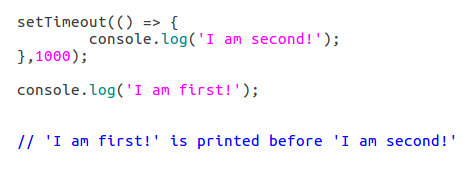
\includegraphics[width=0.6\linewidth]{cb1.png}
  \caption{Example of a callback function}
\end{subfigure}%
\begin{subfigure}[t]{.7\textwidth}
  \centering
  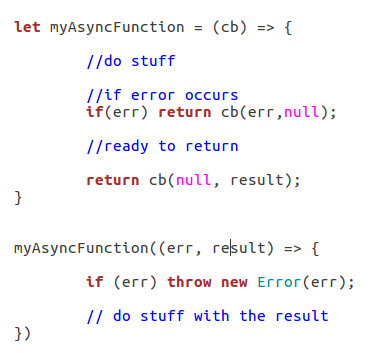
\includegraphics[width=0.6\linewidth]{cb2.png}
  \caption{Example of the callback pattern}
\end{subfigure}
}
\caption{Callback examples}
\label{cbFig}
\end{figure} 

In the framework we developed, we make use of javascript in both front and back end. This programming language uses asynchronous logic, which takes place through the usage of asynchronous callback functions. A callback function, also known as a higher-order function, is a function that is passed to another function (e.g "first") as a parameter, and the callback function is called (or executed) inside the first function. A callback function is essentially a pattern (an established solution to a common problem), and therefore, the use of a callback function is also known as a callback pattern. The execution of the first function does not block the execution of the rest of the program commands. The execution of the callback function begins, when the execution of the first function is completed. An example of node.js callback function pattern can be seen in figure ~\ref{cbFig}. \par
	In our framework, the callback functions are used constantly, so that the design and implementation are transformed accordingly. As a convention, all the callback functions receive as arguments two objects, the error and the result object. Before the execution of the callback function, in case an error occurs, the execution stops and the error object is passed to the callback. The result object is undefined. If no errors occur, the error object is undefined and the result object contains the function outcome. Following we describe two design patterns, which are based in callback functions and are heavily used in the framework implementation.

\subsection{Closures}
\begin{figure}
	\centerline{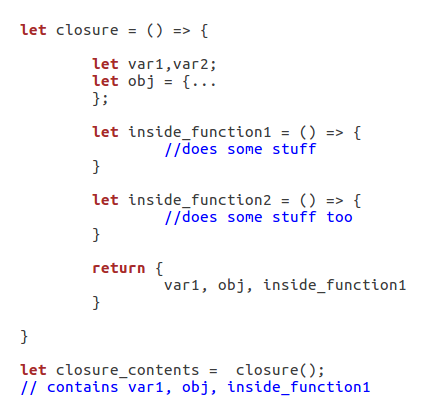
\includegraphics[scale=0.7]{closure.png}}
	\caption{Example of a closure function}
	\label{closure}
\end{figure} 
Javascript is an object oriented language and was created to perform well in any platform. Thus, it has many ways of defining certain structures, such as constructor functions. In our framework, we define our constructors through the closure design pattern. Closures fully implement a constructor functionality.\par
	Generally, a closure in javascript is a function. This function receives arguments that initialize its state. The function body defines contents, such as variables, objects and other functions. Finally, the function returns, or exposes in the rest of the framework, only what is necessary. This may include also variables, objects and functions. Anything that is not returned, is defined as private. An example of this pattern is shown in figure ~\ref{closure}.

\subsection{Thunks}
\begin{figure}
	\centerline{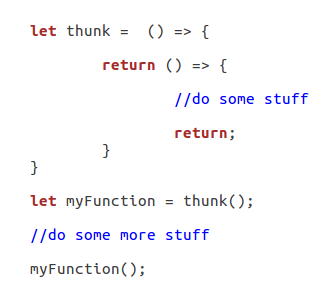
\includegraphics[scale=0.7]{thunk.png}}
	\caption{Example of a thunk function}
	\label{thunk}
\end{figure} 
The thunk pattern has a similar structure with closure, but it's used in a different way. Basically, it's a function which returns another function. The interesting part is that the execution of the first function does not imply the execution of the second. In this way we define "lazy" functions, that is methods which are scheduled to execute but don't until they have to. Thus, asynchronicity is encapsulated, aiding composability and avoiding the "callback hell" problem. This problem is caused by the generation of large sequences of nested callback functions, which is considered a bad design practice and creates debug problems. An example of the thunk pattern is shown in figure ~\ref{thunk}.

\section{Back End implementation}
In this section, we focus in the back end implementation of the framework. Initially we present the REST API and then we describe the development stages of the framework modules. We emphasize in the technologies used and their in between communication (interoperability).

\subsection{REST API}
An important part of the back end framework implementation is the development of the REST API, which is achieved through routing. Routing refers to determining how an application responds to a client request for a specific endpoint, which is a URI (or path) and a specific HTTP request method (GET, POST, PUT or DELETE). Each of our routes has different handler functions which are executed when the route is matched. The route handler functions use the information which is given to them through the request, and after the execution of internal operations, return a response object to the client.\par
	 The response object has a concrete structure and includes all the required information. Among other things, it contains the status code and the result data. Generally the content of the response object is determined by the request method and the success of the operation (error handling is described thoroughly in chapter ~\ref{errorHandling}). The structure of the response object implements the JSON format. \par 
	 	Following we present all the routes for each model entity seperately. For some of them we describe their corresponding handlers.
	 	
\paragraph{}
\begin{table}[]
\centering
\begin{tabular}{|c|c|}
\hline
\rowcolor[HTML]{32CB00} 
\textbf{URI}     & \textbf{method} \\ \hline
\rowcolor[HTML]{FFFFFF} 
/login           & GET             \\ \hline
\rowcolor[HTML]{67FD9A} 
/logout          & GET             \\ \hline
\rowcolor[HTML]{FFFFFF} 
/isauthenticated & GET             \\ \hline
\end{tabular}
\caption{Authentication URI's}
\label{authURI}
\end{table}
The routes of the table ~\ref{authURI} are used by the framework for the authentication of the users. The login route checks whether the client's credentials exist in an instance of the users model of the database. If the client is identified, a positive confirmation is sent to the user, while at the same time a session cookie is saved (session management is described in chapter ~\ref{security}). Otherwise, the server's response is negative. The logout route disconnects the user from the framework and its corresponding session cookie is deleted from the database. The last route is used from the framework to check if the user is already authenticated. If this event occurs, the authentication step is skipped.

\paragraph{Users}
\begin{figure}
	\centerline{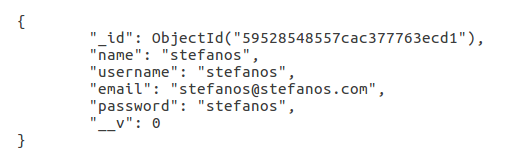
\includegraphics[scale=0.7]{userObject.png}}
	\caption{Example of a User instance}
	\label{userObject}
\end{figure}
\begin{table}[]
\centering
\begin{tabular}{|c|c|c|}
\hline
\rowcolor[HTML]{32CB00} 
\textbf{Model} & \textbf{URI}                                                     & \textbf{method}                                     \\ \hline
\rowcolor[HTML]{FFFFFF} 
Users          & /users/?id=\{user\_id\}                                              & GET                                                 \\ \hline
\rowcolor[HTML]{67FD9A} 
Users          & /register                                                        & POST                                                \\ \hline
\rowcolor[HTML]{FFFFFF} 
Users          & /users/?id=\{user\_id\}                                              & PUT                                                 \\ \hline
\rowcolor[HTML]{67FD9A} 
Users          & \multicolumn{1}{l|}{\cellcolor[HTML]{67FD9A}/users/?id=\{user\_id\}} & \multicolumn{1}{l|}{\cellcolor[HTML]{67FD9A}DELETE} \\ \hline
\end{tabular}
\caption{Users URI's}
\label{usersURI}
\end{table}
Table ~\ref{usersURI} presents the routes which concern the users model. The POST method is responsible for the creation of new user instances. It checks whether all fields have a value and, the username and email properties are unique. The figure ~\ref{userObject} presents the structure of a User instance. The GET method returns the user instance information and the projects in which he participates. The PUT and DELETE methods are used for their corresponding functionalities.

\paragraph{Projects}
\begin{figure}
	\centerline{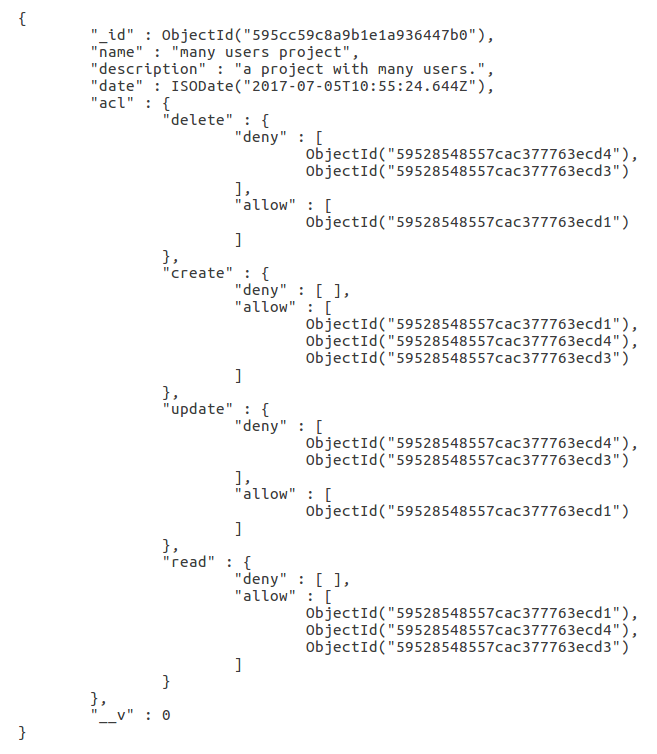
\includegraphics[scale=0.7]{projectObject.png}}
	\caption{Example of a Project instance with three users}
	\label{projectObject}
\end{figure}
\begin{table}[]
\centering
\begin{tabular}{|c|c|c|}
\hline
\rowcolor[HTML]{32CB00} 
\textbf{Model} & \textbf{URI}                   & \textbf{method} \\ \hline
\rowcolor[HTML]{FFFFFF} 
Projects       & /projects/?id=\{project\_id\}      & GET             \\ \hline
\rowcolor[HTML]{67FD9A} 
Projects       & /projects                      & POST            \\ \hline
\rowcolor[HTML]{FFFFFF} 
Projects       & /projects/join/?id=\{project\_id\} & GET             \\ \hline
\end{tabular}
\caption{Projects URI's}
\label{projectsURI}
\end{table}
The Project model REST API is presented in table ~\ref{projectsURI}. The POST method is used for the creation of project model instances. The  figure ~\ref{projectObject} presents the structure of a Project instance. The GET method searches out for a specific project and its elements. Then the datasets and posts which are related to the projects, are returned along with the project information. The join route is responsible for the addition of project members. In order to implement it, an update of the ACL property of the project instance takes place.

\paragraph{Datasets}
\begin{table}[]
\centering
\begin{tabular}{|c|c|c|}
\hline
\rowcolor[HTML]{32CB00} 
\textbf{Model}                                         & \textbf{URI}                                                               & \textbf{method}                                     \\ \hline
\rowcolor[HTML]{FFFFFF} 
Datasets                                               & /datasets/?id=\{dataset\_id\}                                              & GET                                                 \\ \hline
\rowcolor[HTML]{67FD9A} 
Datasets                                               & /datasets                                                                  & POST                                                \\ \hline
\rowcolor[HTML]{FFFFFF} 
Datasets                                               & /datasets/list/?id=\{dataset\_id\}                                         & GET                                                 \\ \hline
\rowcolor[HTML]{67FD9A} 
Datasets                                               & /datasets/grid/?id=\{dataset\_id\}                                         & GET                                                 \\ \hline
\rowcolor[HTML]{FFFFFF} 
\multicolumn{1}{|l|}{\cellcolor[HTML]{FFFFFF}Datasets} & \multicolumn{1}{l|}{\cellcolor[HTML]{FFFFFF}/datasets/?id=\{dataset\_id\}} & \multicolumn{1}{l|}{\cellcolor[HTML]{FFFFFF}DELETE} \\ \hline
\end{tabular}
\caption{Datasets URI's}
\label{datasetsURI}
\end{table}
The routes of the table ~\ref{datasetsURI} are developed for the Datasets model. A general analysis of the dataset save and retrieval management is described in chapter ~\ref{pyfiles}. The GET method returns the contents of an HDF file. The POST and DELETE methods are responsible for the creation and deletion of a dataset, respectively. The list route returns a list of datasets, which are contained in a project. Also, the grid route returns a chunk of an array, which is located inside a dataset, in order to present it to the client.

\paragraph{Posts}
\begin{table}[]
\centering
\begin{tabular}{|c|c|c|}
\hline
\rowcolor[HTML]{32CB00} 
\textbf{Model} & \textbf{URI}            & \textbf{method} \\ \hline
\rowcolor[HTML]{FFFFFF} 
Posts          & /posts/?id=\{post\_id\} & GET             \\ \hline
\rowcolor[HTML]{67FD9A} 
Posts          & /posts                  & POST            \\ \hline
\rowcolor[HTML]{FFFFFF} 
Posts          & /posts/?id=\{post\_id\} & UPDATE          \\ \hline
\rowcolor[HTML]{67FD9A} 
Posts          & /posts/?id=\{post\_id\} & DELETE          \\ \hline
\end{tabular}
\caption{Posts URI's}
\label{postsURI}
\end{table}
\begin{figure}
	\centerline{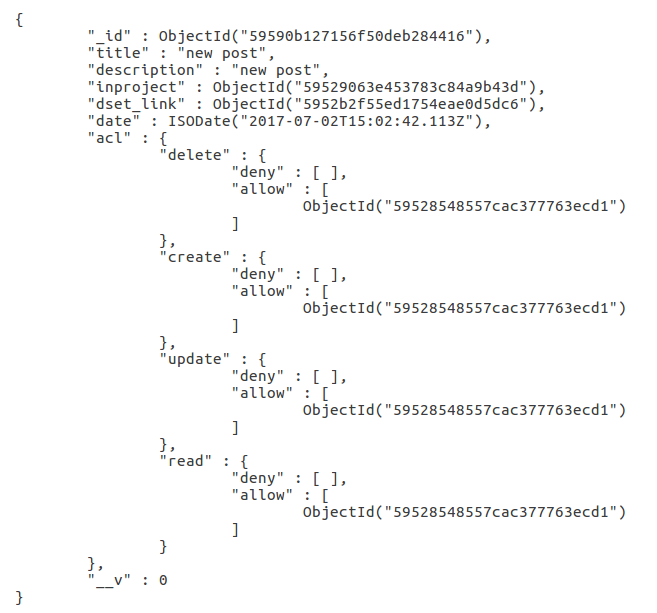
\includegraphics[scale=0.7]{postObject.png}}
	\caption{Example of a Post instance}
	\label{postObject}
\end{figure}
Table ~\ref{postsURI} presents the routes which are related to the posts model. All the methods are used for the corresponding functionalities. The figure ~\ref{postObject} presents the structure of a Post instance. 

\paragraph{Plots}
\begin{table}[]
\centering
\begin{tabular}{|c|c|c|}
\hline
\rowcolor[HTML]{32CB00} 
\textbf{Model} & \textbf{URI}            & \textbf{method} \\ \hline
\rowcolor[HTML]{FFFFFF} 
Plots          & /plots/?id=\{plot\_id\} & GET             \\ \hline
\rowcolor[HTML]{67FD9A} 
Plots          & /plots                  & POST            \\ \hline
\rowcolor[HTML]{FFFFFF} 
Plots          & /plots/?id=\{plot\_id\} & DELETE          \\ \hline
\end{tabular}
\caption{Plots URI's}
\label{plotsURI}
\end{table}
\begin{figure}
	\centerline{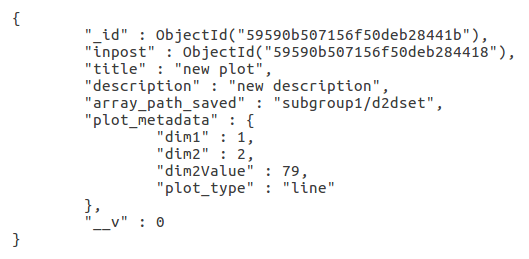
\includegraphics[scale=0.7]{plotObject.png}}
	\caption{Example of a Plot instance}
	\label{plotObject}
\end{figure}
The Plot model REST API is presented in table ~\ref{plotsURI}. All the methods are used for the corresponding functionalities. The figure ~\ref{plotObject} presents the structure of a Plot instance. 


\subsection{NoSQL Access Management}
In chapter ~\ref{nosql} a thorough description of the design of the NoSQL access module is presented. In this chapter we mention the technologies we used and the implementation of this module. \par
	A standard library we use in this module is Mongoose.js. This library offers  a schema based solution in the modelling of the database for node.js. It grants complete CRUD operations which we use in data access object module. These operations are developed as callback functions, so the execution of the function does not stop the code flow. When the execution of a CRUD operation is completed, a callback function is called. Also, the data communication between the internal modules and the mongoose library is implemented through javascript objects.

\subsection{Security Management}
\label{security}
In chapter ~\ref{def} we present the general idea of the security design. Here we describe how these modules are combined to implement the security objective. The technologies we use are presented too. Initially, we introduce the passport javascript module, which has the key role in session management. \par
	Passport is a node.js library which is used for the user authentication. When a user logs in the framework, the library creates a cookie object which is saved in a database collection. Furthermore, it embodies this cookie in the respond object, which is sent to the client. This operation is called serialization. The client saves the cookie object and sends it back to the future requests. When the user logs out or a certain amount of time has passed without connecting to the system, the passport library deletes the user cookie from the database. This operation is called deserialization. The framework ensures the correct communication between the login- logout routes and their corresponding handlers, the passport library and the database collection. \par 
	The defender middleware module combines the authentication/session management functionality we described above, with the authorization functions that are introduced in the noSQL access module. Initially, the system investigates if the request object includes the required cookie, so that the authentication can be completed. If the operation succeeds, the request object URI is examined. With some exceptions, the URI's first part corresponds to one of the models  the database provides. Also, the request method must be one of GET, POST, UPDATE or DELETE. \par 
	The last part of the security module is the authorization investigation of the framework. As mentioned in chapter \ref{nosql}, the functionality of the permissions model includes functions which investigate permissions of a model instance. At this point we use isAllowed and isAllowedCreate functions to check if the request is allowed to proceed. If the examination is successful, the middleware operation is completed and the routes module is called. In all situations that the check fails, the access is denied for the user and a corresponding status code is returned (401 if not authenticated and 403 if not authorized).

\subsection{Python - Node.js Interoperability}
As aforementioned in chapter ~\ref{hdf}, HDF is an essential ingredient of the framework for storing multidimensional datasets. The HDF library is developed in C/C++, which constitutes it as foreign code to our framework. Firstly we studied ways of embedding foreign code in node.js. An option for establishing inter-processing communication (IPC) is over Standard Input/Output (STDIO), available in all major operating systems.\par 
	Although an opensource project which exposes the HDF functionality directly to node.js exists, we observed prohibitive inefficiencies in its implementation. Thus, we set upon a more mature python implementation, the h5py. A module responsible for sending messages from our framework to h5py, and inversely, was developed. The rest of this section is dedicated to the way this module operates.\par 
	Node.js includes a spawn functionality of the child process module, which allows invocation of external processes, parameterized by arguments. The results of the python execution are manipulated by the event listener, returned by the child process. The controller listens for the data and error events. In case of an error, a new error object is propagated, while in the opposite case the result is parsed. \par 
	We use the included python's JSON library, which enables easy information parsing to a javascript object. Via the STDOUT buffer, all the results are serialized and accessed from javascript. We design a communication protocol between python and node.js, for the customization of the script functions. Python executes the corresponding commands, returning successful results or potential errors.


\section{Front End Implementation}
In this section we continue with the description of the front end part of the implementation. While initially we investigated different framework options for the client tier, we ended up using pure javascript. We considered overkill the usage of a large framework for our requirements. This way we pursued the better understanding of javascript's front end functionality. In addition, it is important to point out that the lack of context switching aids productivity, when using javascript end to end. We were satisfied with the usage of small libraries, whenever it was necessary. \par 
	A fundamental characteristic of our framework's front end is the single page application design approach, as explained in chapter ~\ref{spa}. According to this architecture, all the essential code is retrieved in the front end in a single page load. Then, the communication between client and server is based entirely in ajax requests (see chapter~\ref{ajax}). In order to implement this approach, we used a library called browserify. This library offers the ability to require files, as node.js uses it. Then it scans and finds all the files which use the require functionality and bundles them in one file, so it can be sent to the client. \par
	This functionality solves many of our problems. Firstly, it's not vital anymore to write all the files inside script tags in the html files one by one, based on the dependency and execution order. But the great advantage is that a corresponding model of the back end is implemented in the front end part of the framework. Thus, a model hierarchy, which includes modules that can be combined and reused, is defined. In this way, a model driven software development design approach is adopted by the client.

\subsection{Code organization and content}
\begin{figure}
	\centerline{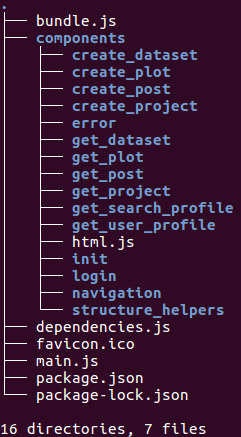
\includegraphics[scale=0.7]{clienttree.png}}
	\caption{Client structure tree}
	\label{clienttree}
\end{figure}
Figure ~\ref{clienttree} represents the general internal structure of the client files. The front end makes use of an approach corresponding to the server and the node.js implementation through the utilization of the node package manager. The package.json file contains vital information for the client network, such as library dependencies, different environment execution scripts etc. The main.js file is the first file to execute, by starting the client's initialization. \par 
\begin{figure}
	\centerline{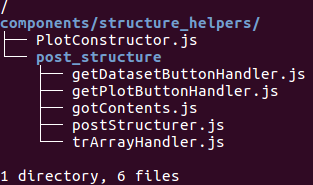
\includegraphics[scale=0.7]{poststructuretree.png}}
	\caption{Post component structure tree example}
	\label{poststructuretree}
\end{figure}
	The components folder includes, among others, all the modules which are executed according to the corresponding user choices. Figure ~\ref{poststructuretree} represents one of these components. It contains submodules responsible for the creation of the appropriate elements. Event handlers modules are also included, in order to manage the functionality of elements, e.g a button. Finally, the component utilizes a module, the purpose of which is the exchange of information between server and client, established via ajax requests.\par
	The communication between the components is secured through the dependencies.js file. This file is received as a parameter in all the components of the client, in order to become available in any case. When the service of a component is terminated, the user interface's content is removed in order to execute another component, which is available through the dependencies.js file.

\paragraph{html.js}
This file is developed to define the front end basic operations, which are related to the html functionality. Starting from core javascript methods, such as createElement or addEventListener, we developed a wrapper adapted to our purpose. The functions create, mountTo and addListenerTo are exposed from this file to the front end and are used constantly in all components. 

\subsection{Plot generation with c3.js}
Plot generation is an essential service of the developed application. In combination with the HDF functionality in the back end, we created a service, through which the users upload their datasets and can visualize them with plots. C3.js is a javascript library, wrapper of D3.js - the core of data visualization tools. This library offers the ability to create simple and minimal diagrams, and supports all simple plot types. \par 
	In order to generate a plot, the arithmetic data must be received and the corresponding configuration must be implemented. The client receives the arithmetic data and the matching metadata in JSON format. After those are parsed, the arithmetic data are prepared for plotting, via the C3 library. The metadata contain useful information, such as the plot type, by means of which we may present our data. \par 
	This library allows us to update the visual plot, which is incredibly useful in front end time saving. Thus, even before the data are received by the client, the corresponding plot presenting process has already started with empty data input. When the data arrive, the plot updates and it is not necessary to create it again. In addition, this logic offers a more smooth experience for the user.
	
\section{Specific framework operations}
In this section we present some parts of the framework which combine the usage of both front and back end.

\subsection{Plot presentation - Zoom functionality}
\begin{figure}
	\centerline{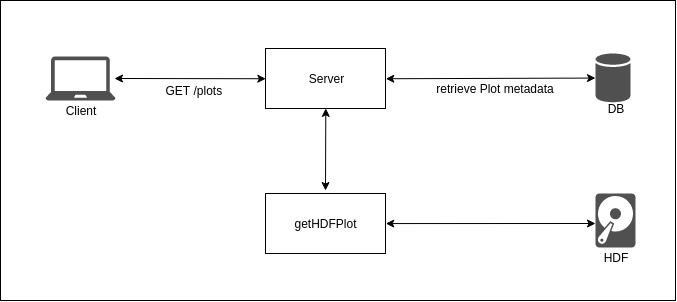
\includegraphics[scale=0.7]{zoom.png}}
	\caption{Plot presentation mechanism}
	\label{zoom}
\end{figure}
In chapter ~\ref{pyfiles} we presented the python scripts which are responsible for the HDF dataset retrieval in JSON format. But how does the plot presentation and zoom functionality operate?\par 
	Figure ~\ref{zoom} presents the actions that must be made inside the framework in order to show a plot to the user. Initially, the user requests the plot display. The front end sends a request, which contains the GET method and the /plot URI, to the corresponding route, along with the specific plot ID. After it is received, the server searches the database for the plot instance and retrieves the related metadata. Following, node.js spawns a new process which executes the getHDFPlot script. This script fetches the HDF file, which contains the plot data, and returns these data in JSON format. Finally, the server is ready to send the result to the client. \par 
	
\begin{figure}
\centering
\begin{subfigure}{1\textwidth}
  \centering
  \centerline{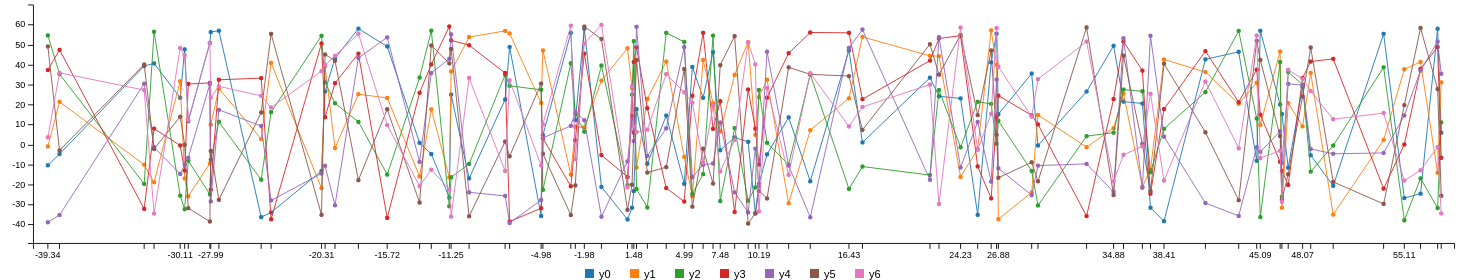
\includegraphics[width=1.2\linewidth]{plotcontentsNOzoom.png}}
  \caption{A plot without zoom}
  \label{fig:sub1}
\end{subfigure}
\begin{subfigure}{1\textwidth}
  \centering
  \centerline{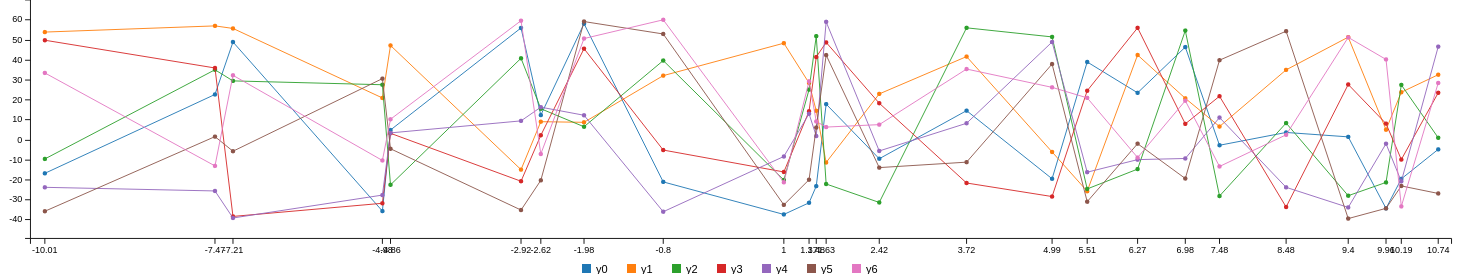
\includegraphics[width=1.2\linewidth]{plotcontentsWITHzoom.png}}
  \caption{A plot with zoom}
  \label{fig:sub2}
\end{subfigure}
\caption{A plot before and after the zoom}
\label{fig:test}
\end{figure}

	To activate the zoom functionality, the user may use the drag and drop mouse technique, to select the first and last point in which he focuses. The corresponding values are sent along the next request as parameters to the server. The procedure is repeated  under the condition that the sampling frequency is calculated based on the parameters distance. The plot which is presented to the user is focused in these specific points.	Figure ~\ref{fig:test} presents the user interface result before and after the zoom.
	
\subsection{Upload functionality}
\begin{figure}
	\centerline{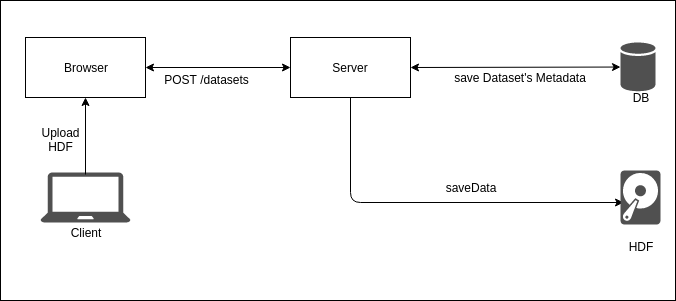
\includegraphics[scale=0.7]{upload.png}}
	\caption{Upload mechanism}
	\label{upload}
\end{figure}
Figure ~\ref{upload} shows the procedure of uploading an HDF file to the framework. Firstly, the file uploads in the browser. Then, the file along with its metadata is sent to the server with a POST method, possibly in chunks of data.  Next, the server checks for the file content, and then saves the HDF file in the filesystem, as explained in chapter~\ref{helpers}. Finally, the file metadata with the unique new filename are saved as a Dataset instance inside the database.

\subsection{Error Handling}
\label{errorHandling}
A very important aspect of the framework is the way through which the system handles its errors. In general, exceptions ~\cite{carlson2000method} are divided in two major categories: those that are created by the client's wrong behaviour, and those that occur from poor software design, also known as bugs. The process by means of which the framework is managing its errors or exceptions of the system, is called error or exception handling. In a framework environment a developer must foresee all the possible exceptions that may occur and provide a handling solution for all of them. The framework must be designed accordingly, by creating a general way of exception handling. \par
	We designed the framework in a way that the handling of an exception happens in the regular flow of the code execution, and not inside a callback function. It is a bad practice to handle the error inside a callback function because the stack trace is lost. We handle the exceptions that occur in the routes and defender modules. All errors are sent with the corresponding status code to the front end. \par 
	 Each time a request to the server is sent by the client, an error check is executed in the response object, in order to handle possible errors. During this check, a potential error is categorized based on the status code, and handled accordingly. In most cases a flash message shows up, but in case of a server error, the error page is presented. \par 
	We pursued the minimization of the number of possible exceptions which occur from the client's wrong behaviour. In order to achieve that, we added in the front end specific conditions, validation restrictions etc, so that it becomes difficult to occur. Also, we implemented a similar logic in the back-end.


\section{Application Presentation}
In this section we briefly present the demo application we created via our framework. Below we show some aspects of the application.

\begin{figure}
\centerline
{
\begin{subfigure}{0.7\textwidth}
  \centering
  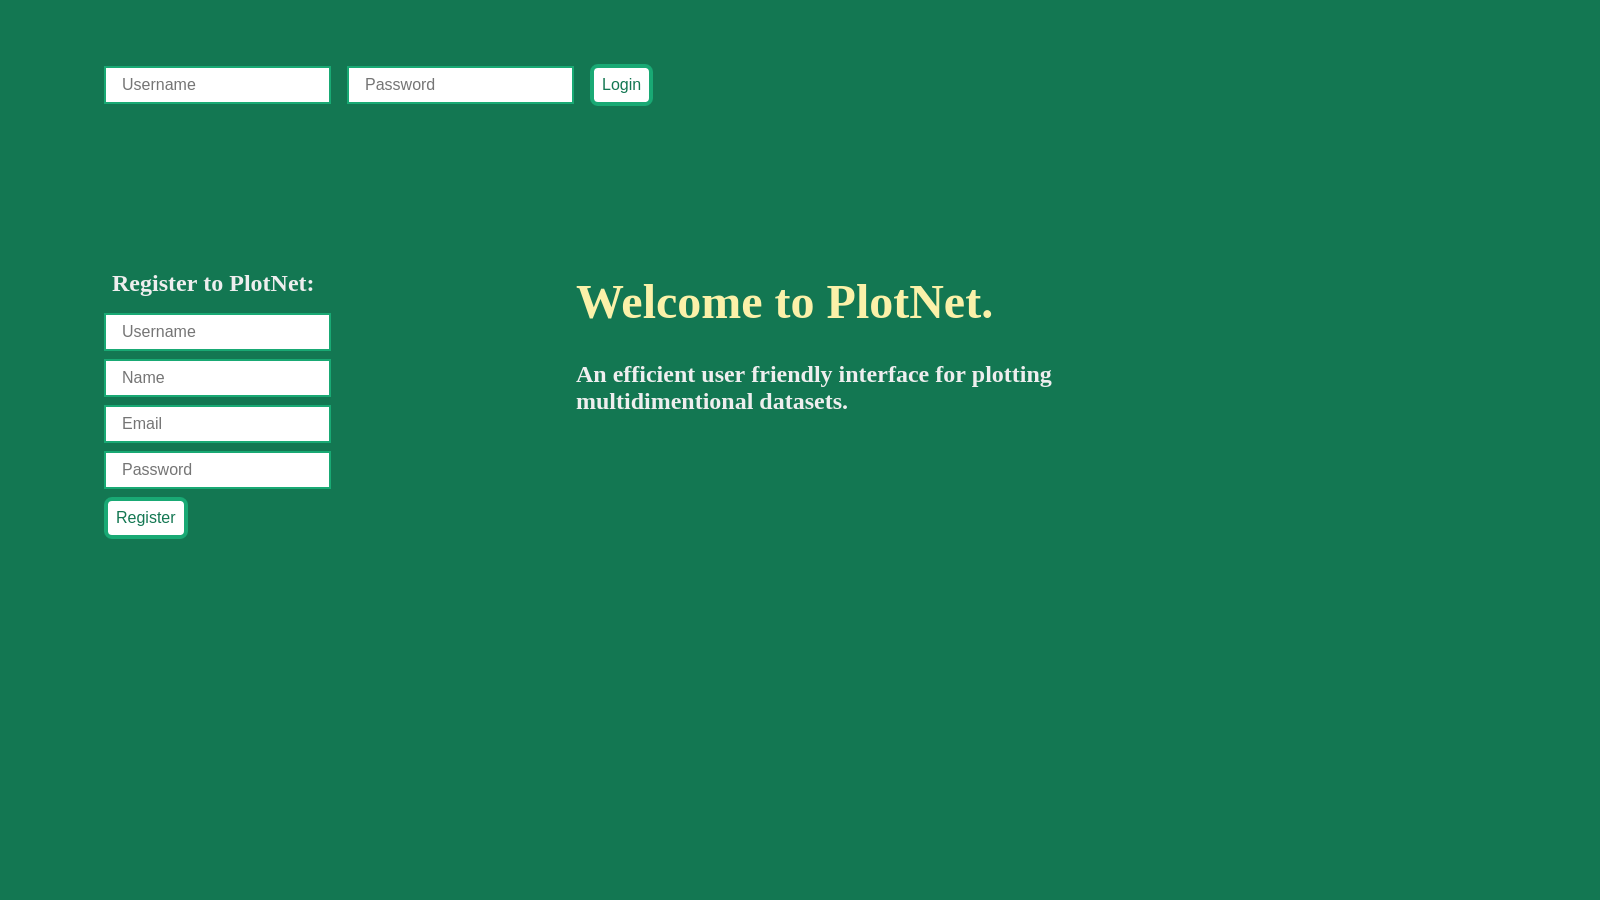
\includegraphics[width=.9\linewidth]{login.png}
  \caption{Login page}
\end{subfigure}%
\begin{subfigure}{0.7\textwidth}
  \centering
  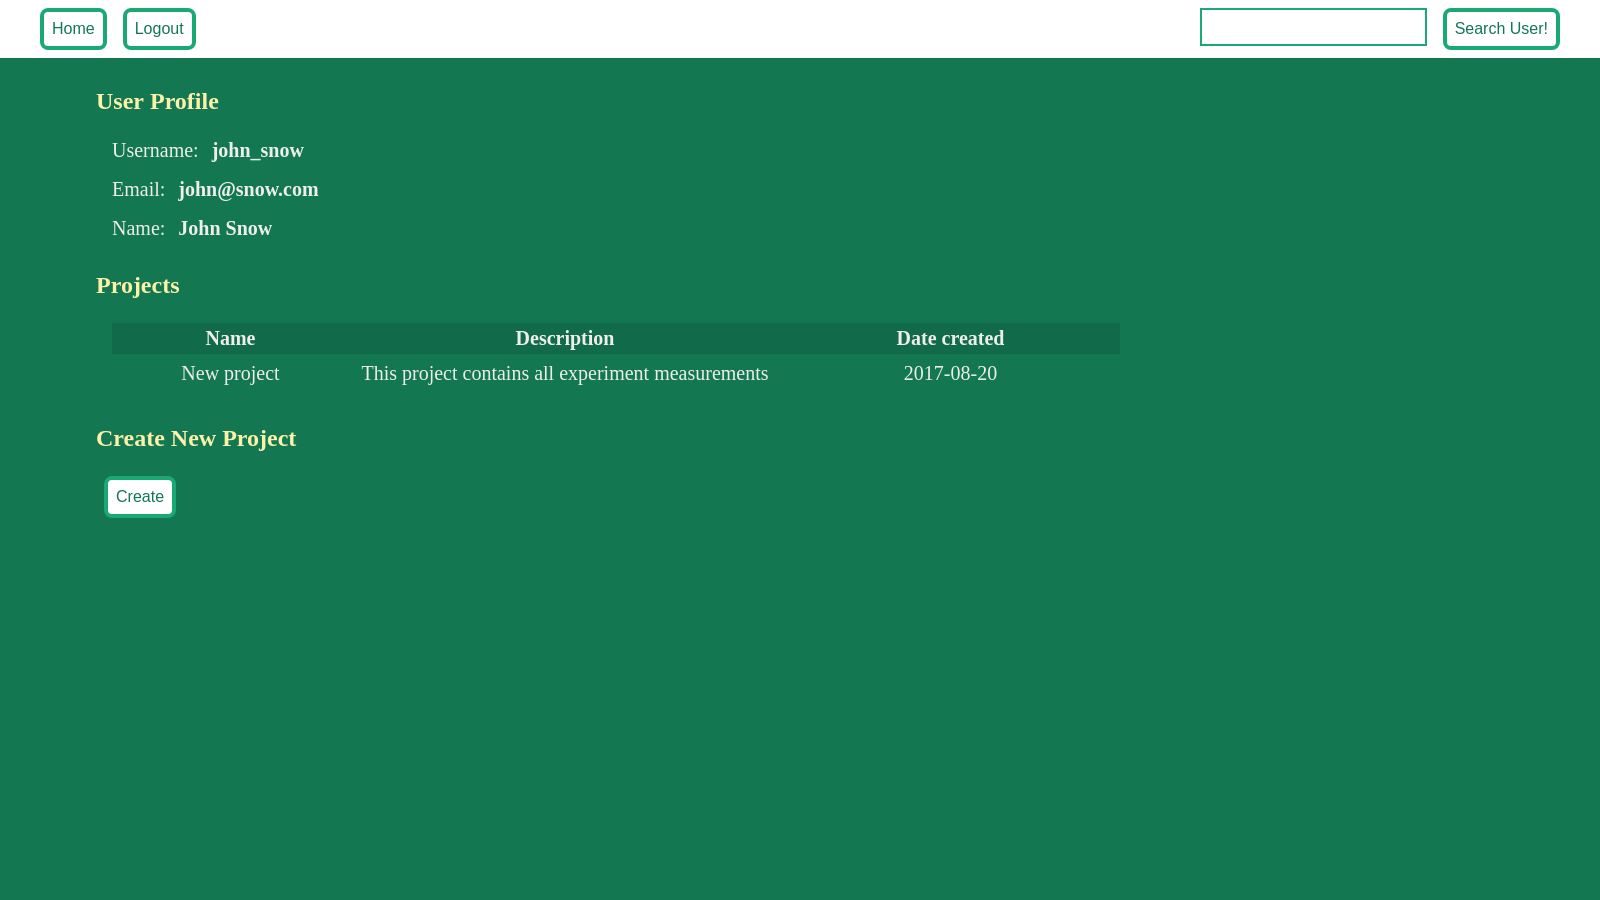
\includegraphics[width=.9\linewidth]{home.png}
  \caption{User home page}
\end{subfigure}}
\centerline
{
\begin{subfigure}{0.7\textwidth}
  \centering
  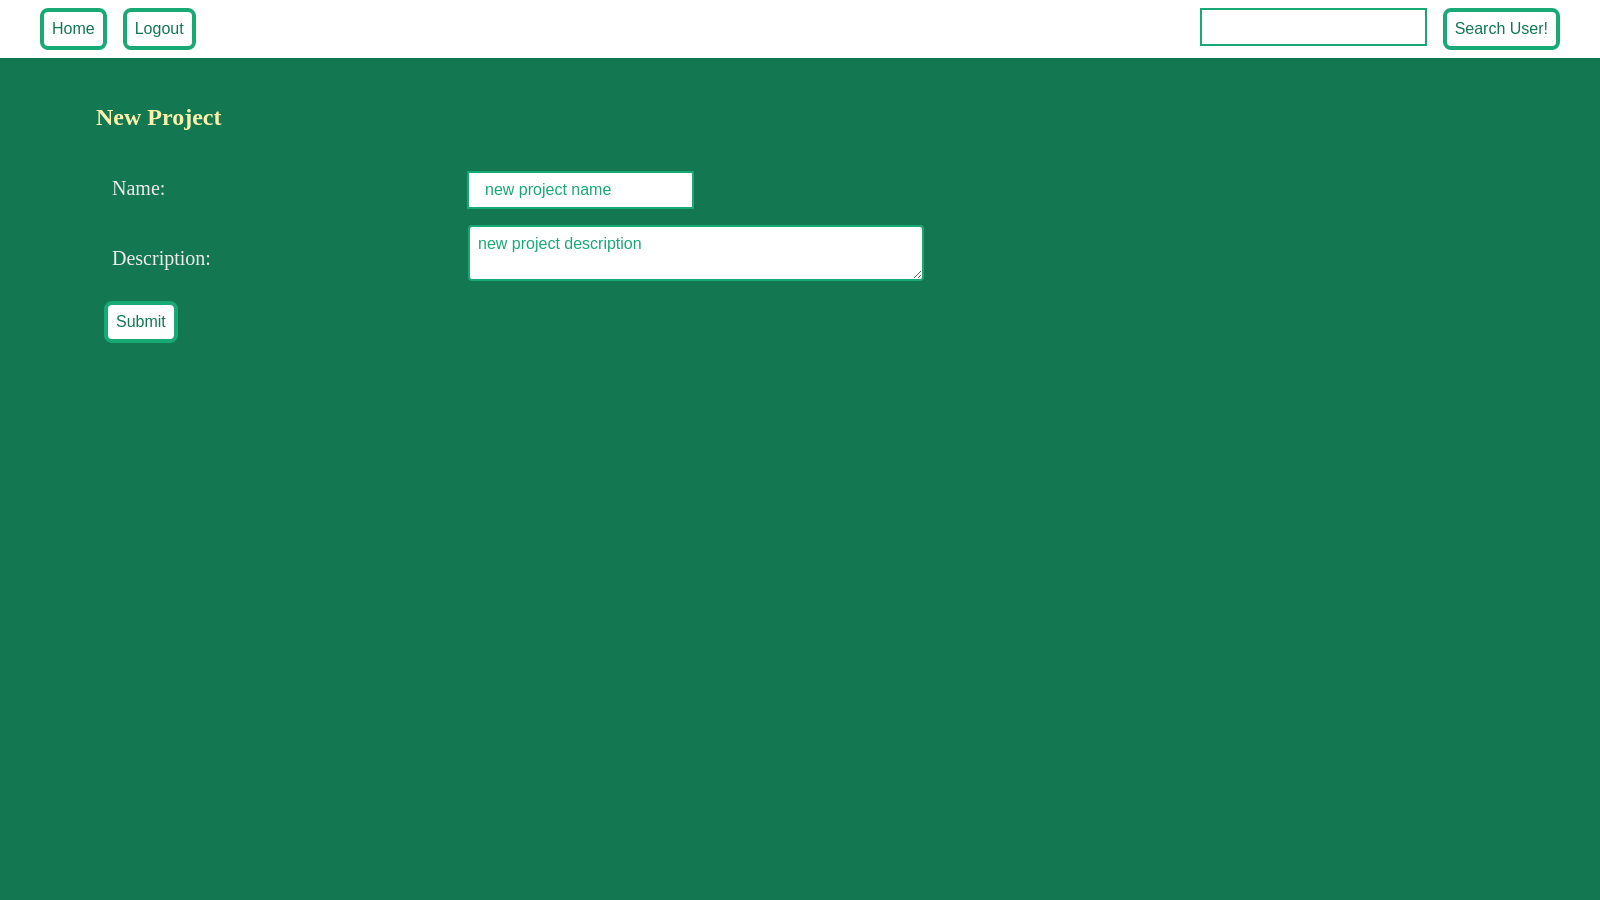
\includegraphics[width=.9\linewidth]{newproject.png}
  \caption{Create new project page}
\end{subfigure}%
\begin{subfigure}{0.7\textwidth}
  \centering
  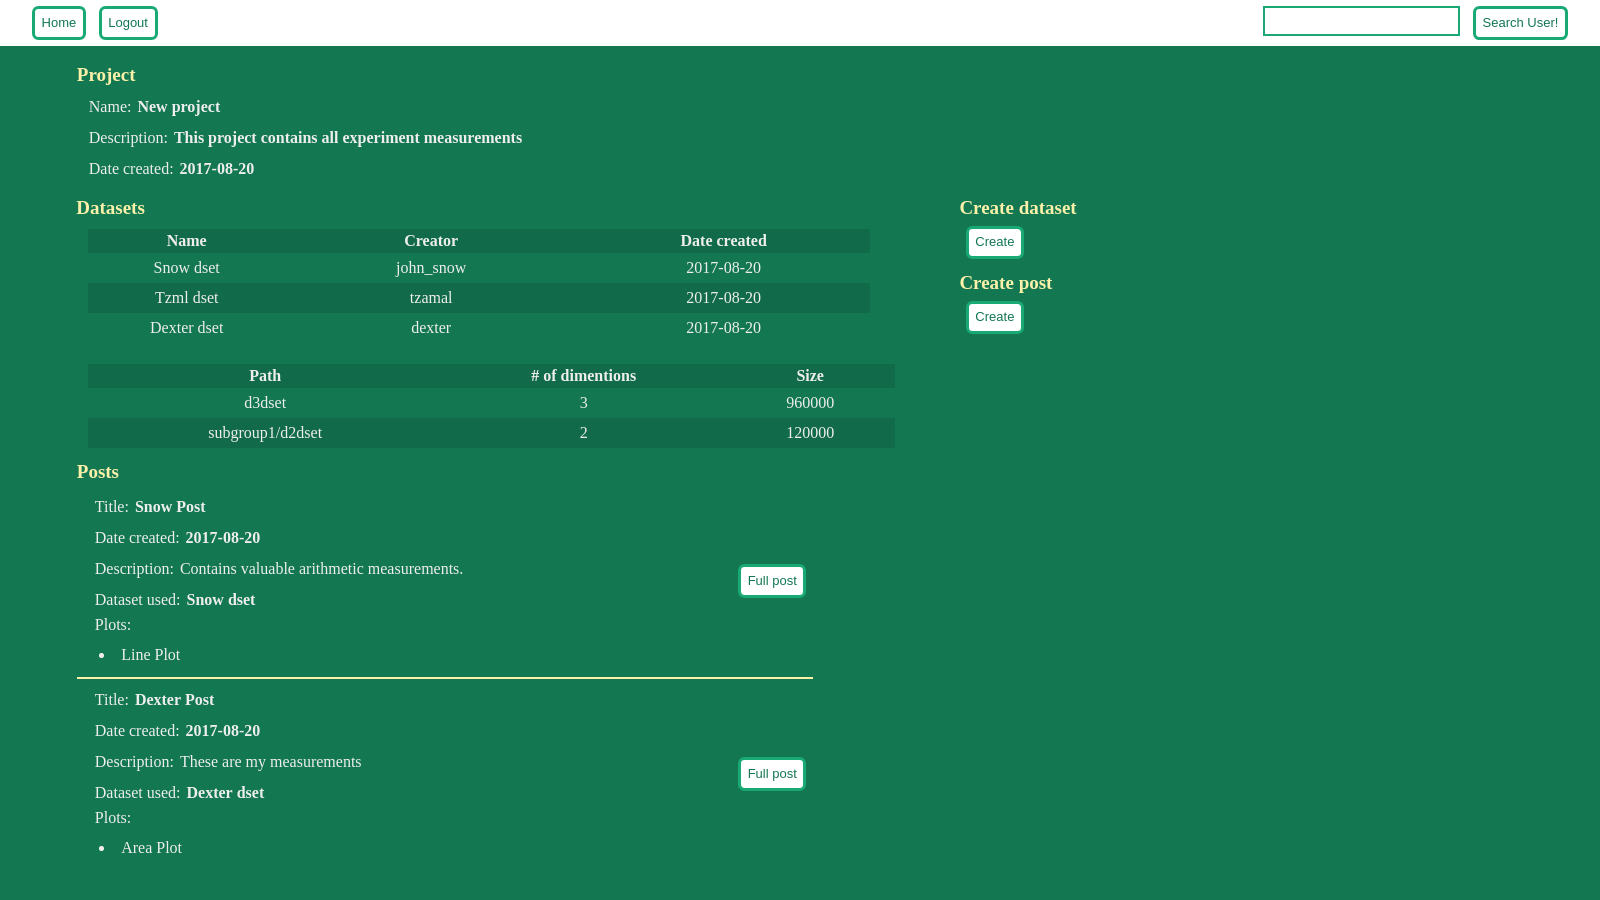
\includegraphics[width=.9\linewidth]{projectcontents.png}
  \caption{Project contents page}
\end{subfigure}
}
\caption{First pages of the application example}
\label{firstfour}
\end{figure}





\begin{figure}
\centerline
{
\begin{subfigure}{0.7\textwidth}
  \centering
  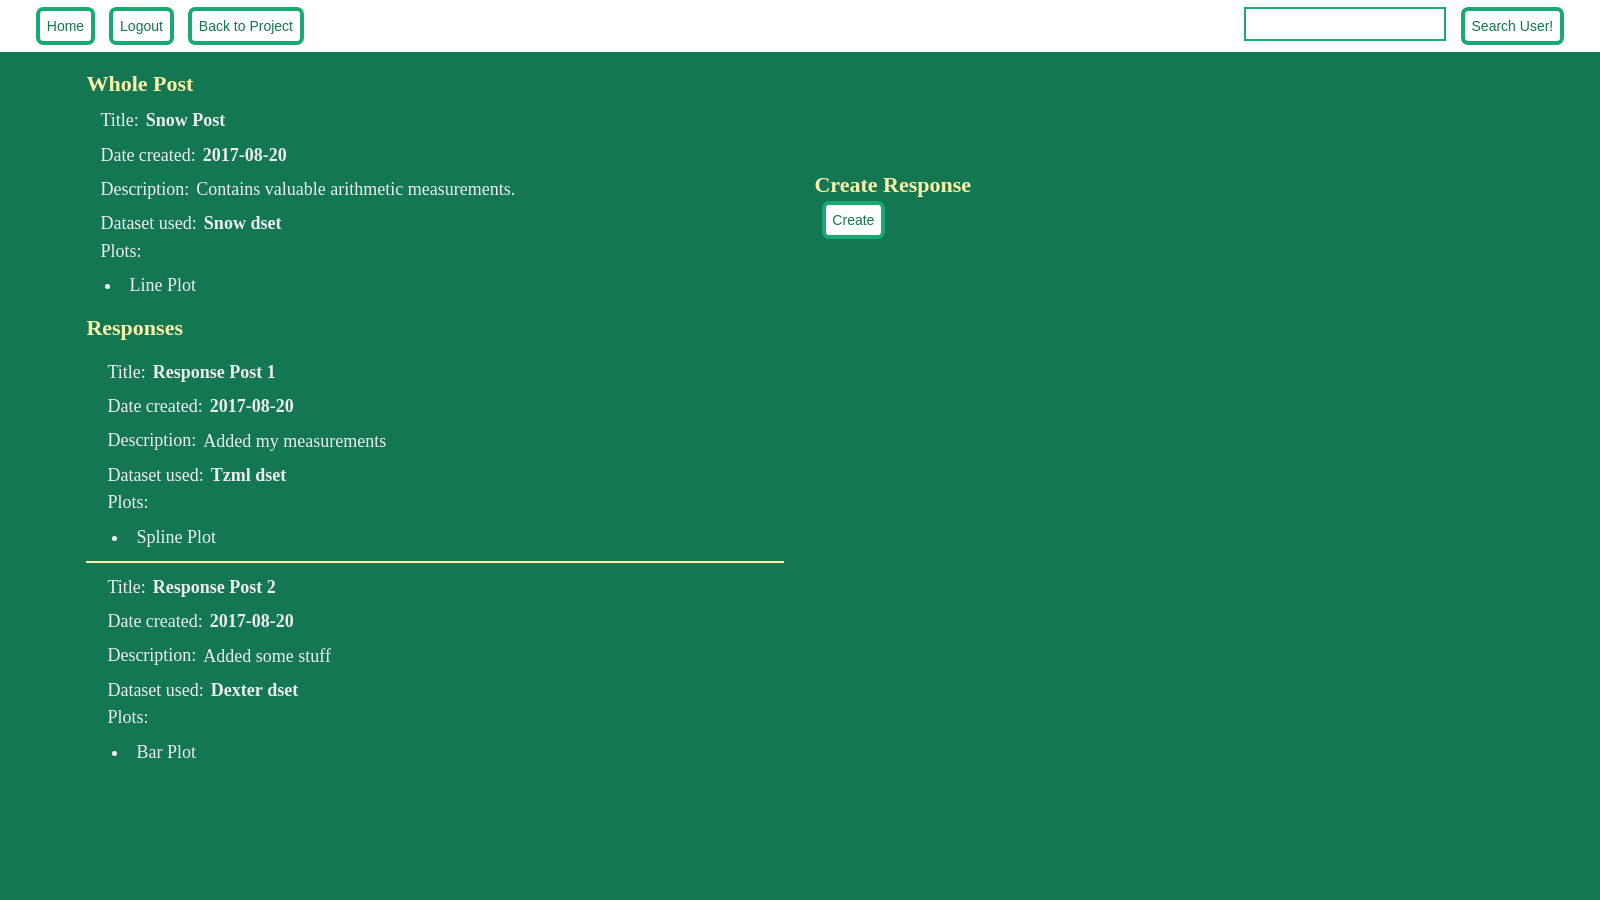
\includegraphics[width=.9\linewidth]{wholepost.png}
  \caption{Show whole post page}
\end{subfigure}%
\begin{subfigure}{0.7\textwidth}
  \centering
  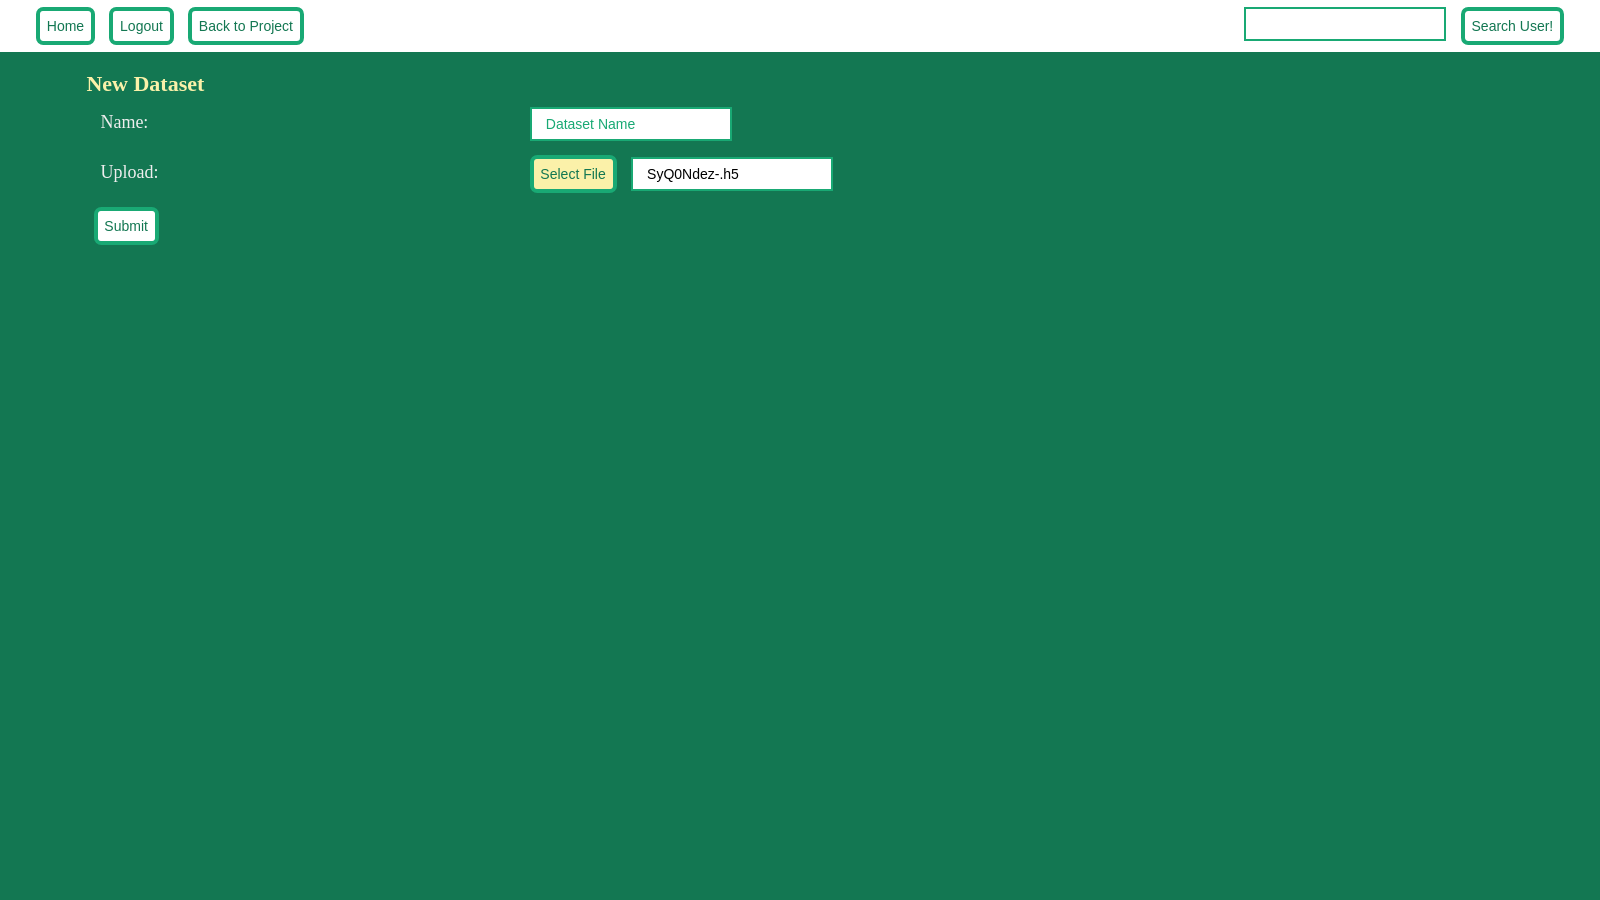
\includegraphics[width=.9\linewidth]{newdataset.png}
  \caption{Create new dataset page}
\end{subfigure}
}
\centerline
{
\begin{subfigure}{0.7\textwidth}
  \centering
  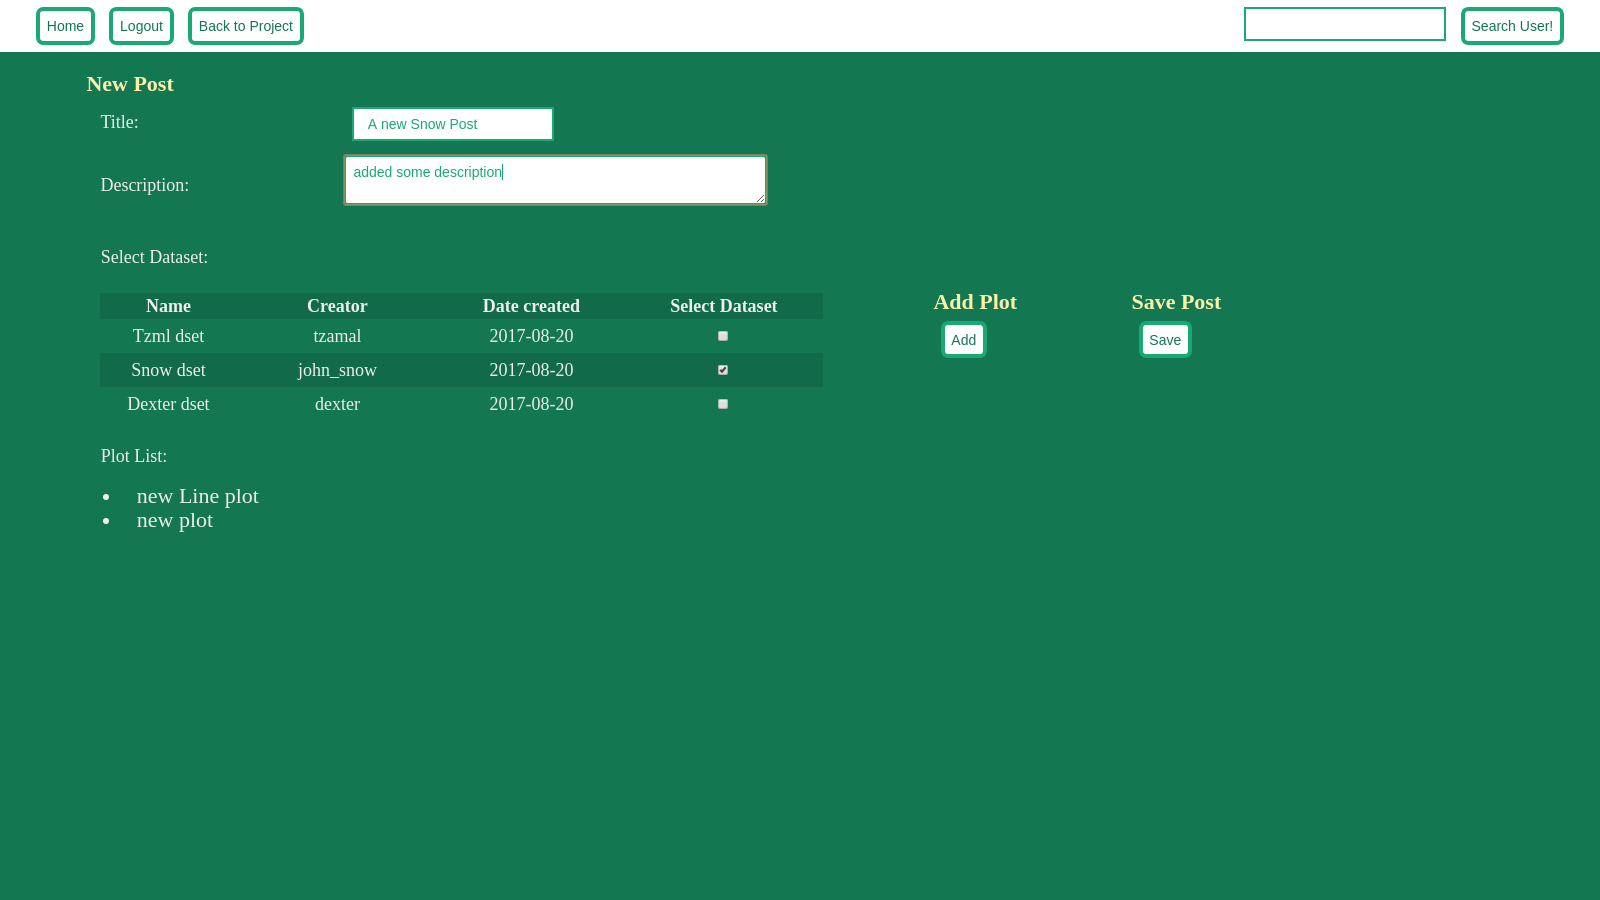
\includegraphics[width=.9\linewidth]{newpost.png}
  \caption{Create new post page}
\end{subfigure}%
\begin{subfigure}{0.7\textwidth}
  \centering
  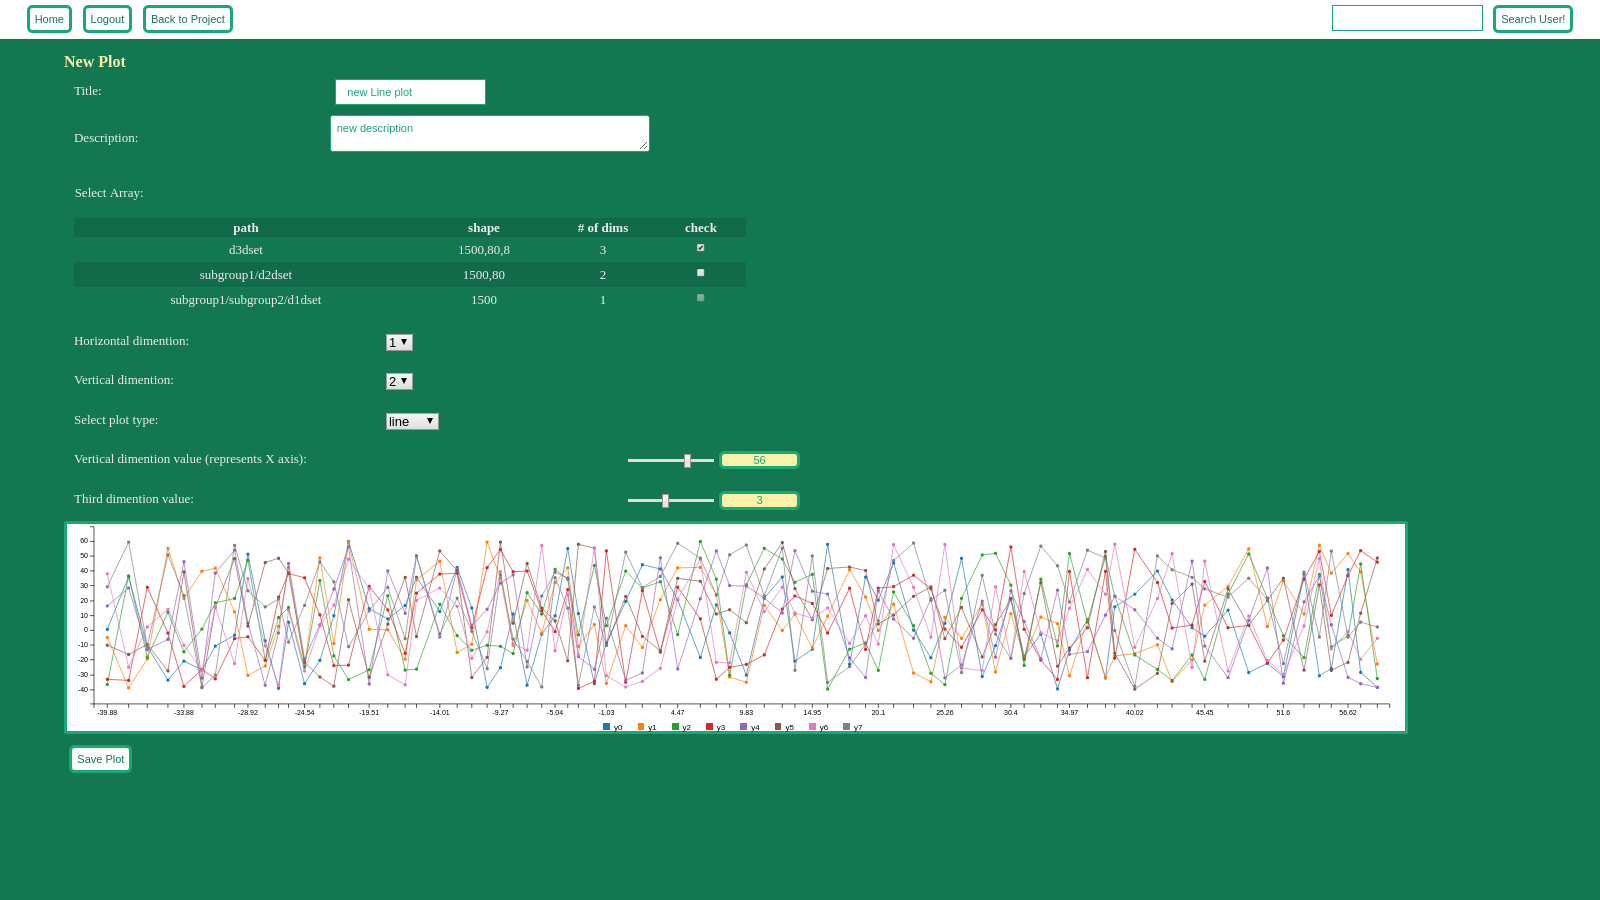
\includegraphics[width=.9\linewidth]{newplot.png}
  \caption{Create new plot page}
\end{subfigure}
}
\caption{Some more pages of the application example}
\end{figure}


\begin{figure}
\centerline
{
\begin{subfigure}{0.7\textwidth}
  \centering
  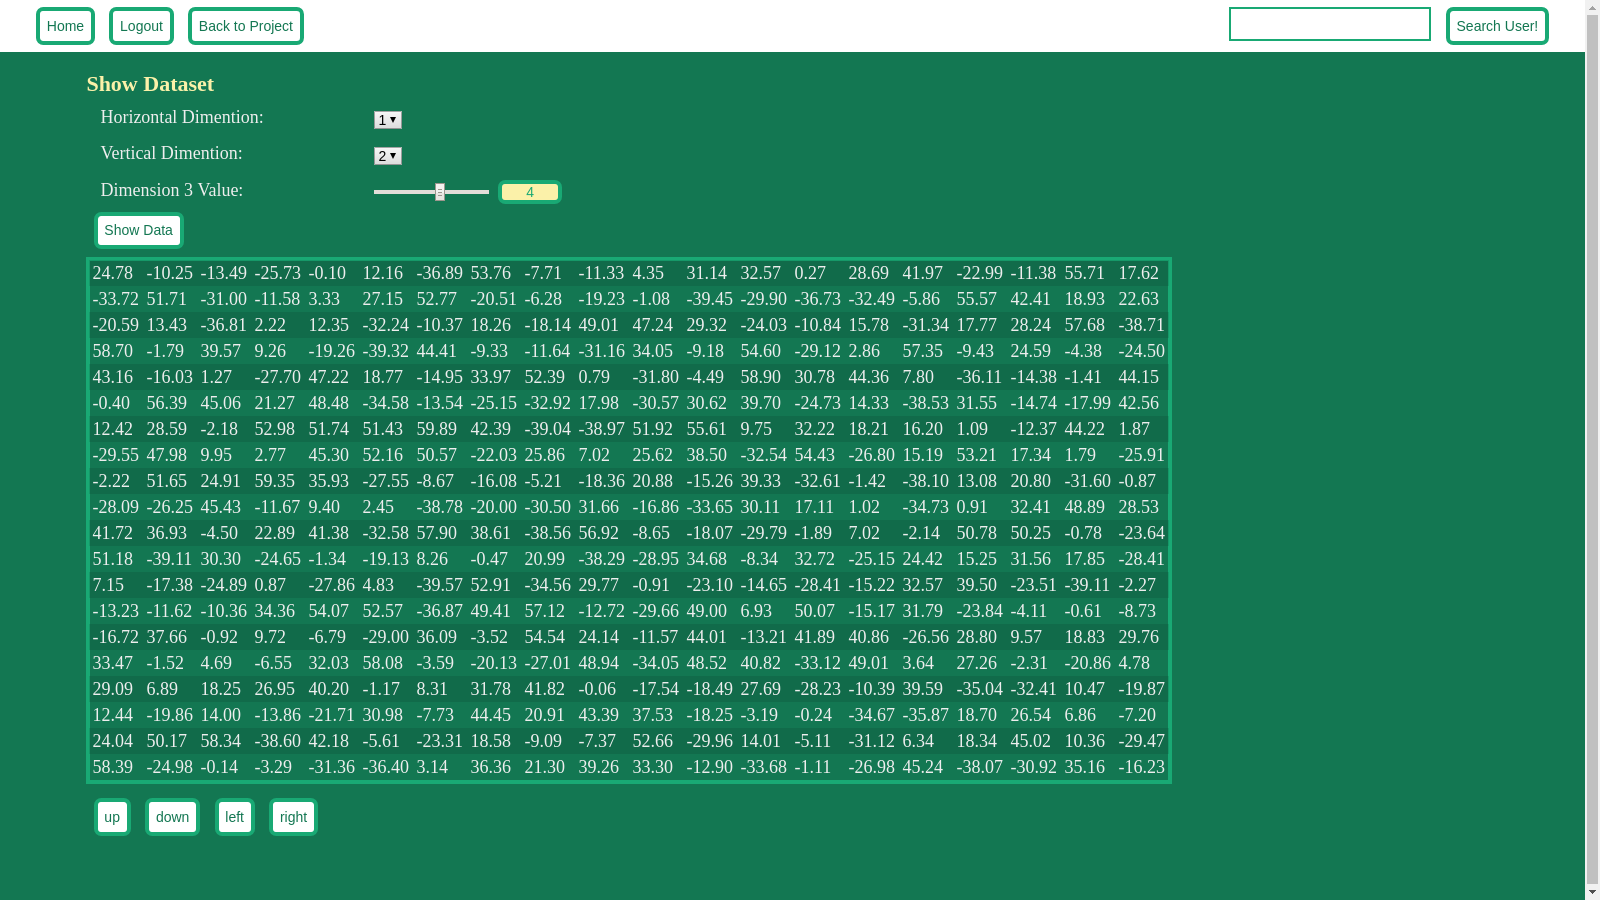
\includegraphics[width=.9\linewidth]{datasetcontents.png}
  \caption{Dataset contents page}
\end{subfigure}%
\begin{subfigure}{0.7\textwidth}
  \centering
  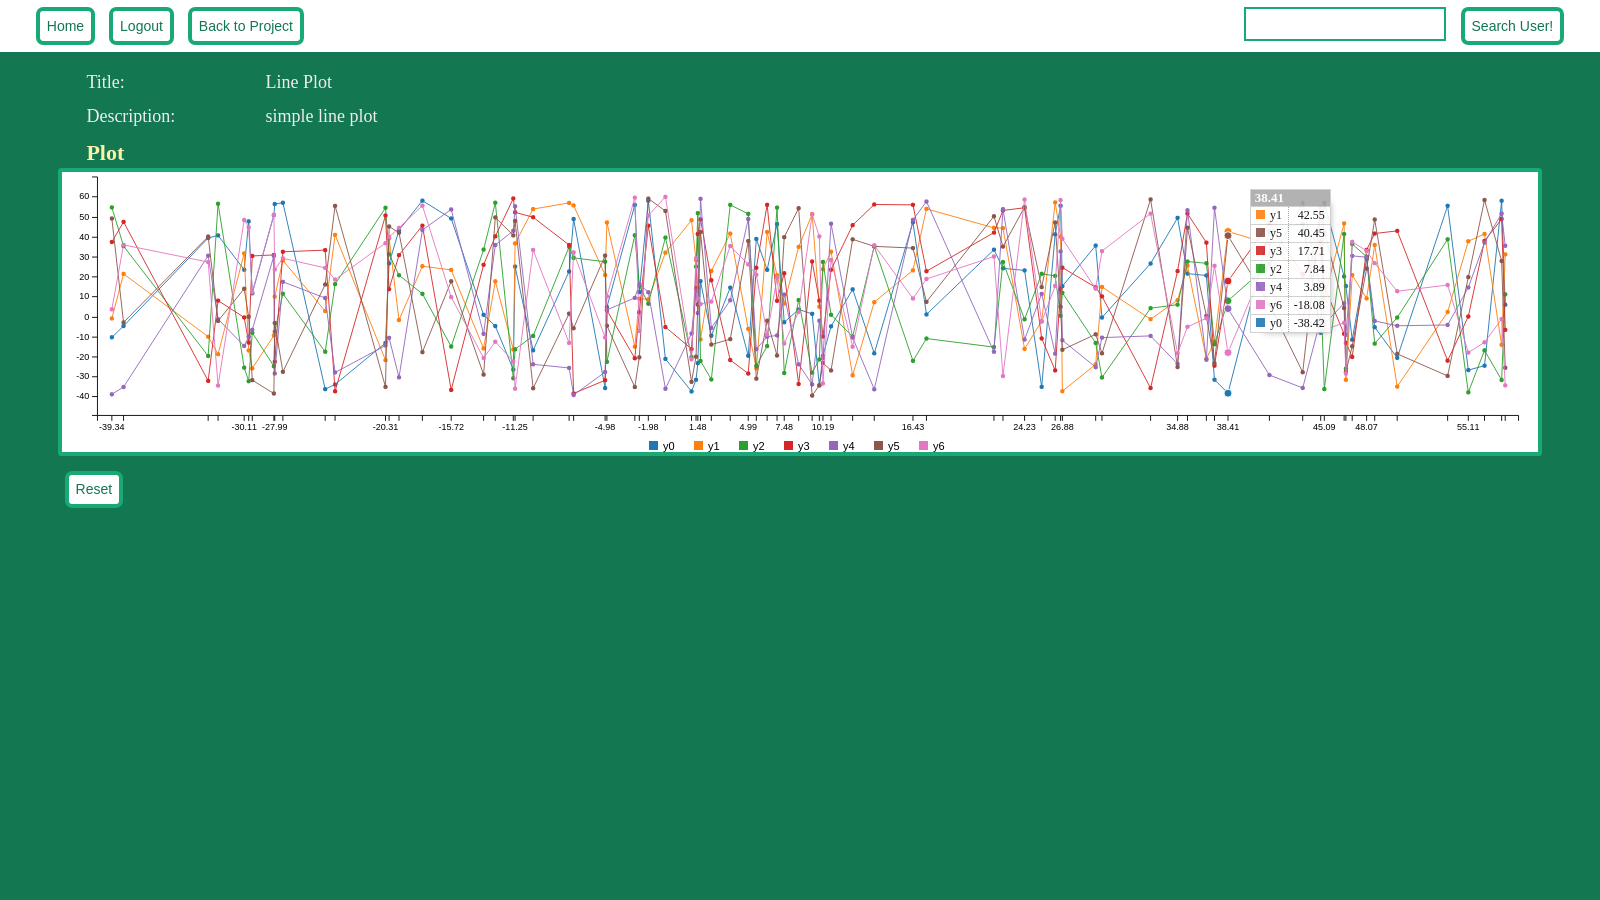
\includegraphics[width=.9\linewidth]{plotcontents.png}
  \caption{Plot contents page}
\end{subfigure}
}
\caption{Last pages presenting dataset and plot contents respectively}
\end{figure}


 
\chapter{Performance Evaluation} % Main chapter title
\label{chapter6_pe}
In this chapter we describe the environment and the test scenarios we implemented in order to record the performance of our system. In table ~\ref{server_ch} we present the characteristics of the server which we use in our tests. \par 
	The capacity of the server's RAM is 8 GB. The operating system we selected for our tests is Debian 8 (Jessie) release. We used two different tools for the benchmarking of our system's performance. The first tool is the ab Apachee HTTP server benchmarking tool, that enables us to send multiple requests  per second with fixed number of total requests. The second tool we used is the wrk, which allows us to send concurrent requests for a specific amount of time with timeout adjustment. With the aid of these tools we implemented two test scenarios, the results of which are presented below. \par 


\begin{table}[]
\centering
\begin{tabular}{|c|c|}
\hline
\rowcolor[HTML]{34FF34} 
\textbf{Architecture}        & x86\_64                              \\ \hline
\rowcolor[HTML]{FFFFFF} 
\textbf{CPU op-mode(s)}      & 32-bit, 64-bit                       \\ \hline
\rowcolor[HTML]{34FF34} 
\textbf{Byte Order}          & Little Endian                        \\ \hline
\rowcolor[HTML]{FFFFFF} 
\textbf{CPU(s)}              & 8                                    \\ \hline
\rowcolor[HTML]{34FF34} 
\textbf{On-line CPU(s) list} & 0-7                                  \\ \hline
\rowcolor[HTML]{FFFFFF} 
\textbf{Thread(s) per core}  & 1                                    \\ \hline
\rowcolor[HTML]{34FF34} 
\textbf{Core(s) per socket}  & 4                                    \\ \hline
\rowcolor[HTML]{FFFFFF} 
\textbf{Model}               & 23                                   \\ \hline
\rowcolor[HTML]{34FF34} 
\textbf{Model name}          & Intel(R) Xeon(R) CPU,X5450,@ 3.00GHz \\ \hline
\end{tabular}
\caption{Server characteristics}
\label{server_ch}
\end{table}


\section{Testing Efficiency in Concurrent Requests}
In the first test we selected some indicative server routes for measurement. In order to measure their performance, we select a predefined number of requests to be sent to the server, changing the number of concurrent requests in each iteration. The criterion of the server's performance is the total time for the response of all the requests. The smaller the time, the better. The results are presented in figure~\ref{experiment_fig}. \par 
 
\begin{figure}
\centering
\begin{subfigure}{1\textwidth}
  \centering
  \centerline{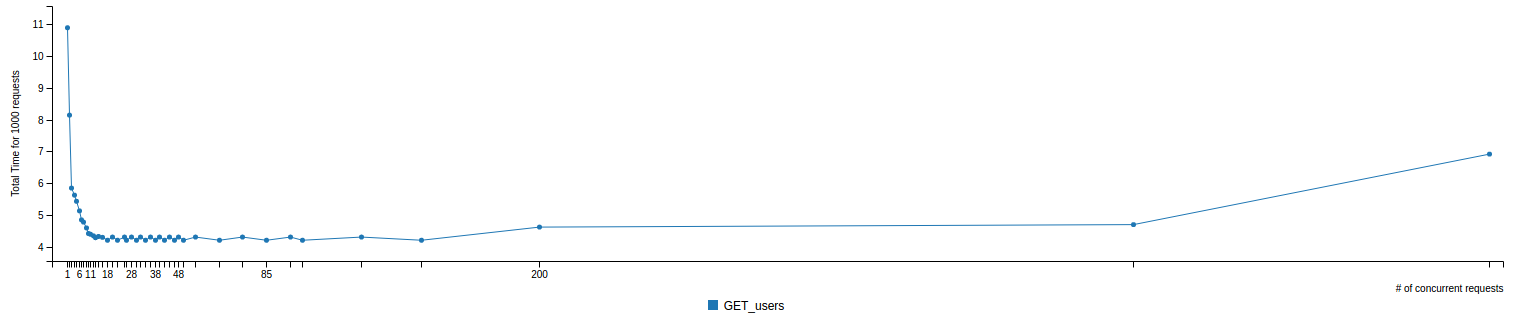
\includegraphics[width=1.2\linewidth]{get_users.png}}
  \caption{GET users route experiment}
\end{subfigure}
\begin{subfigure}{1\textwidth}
  \centering
  \centerline{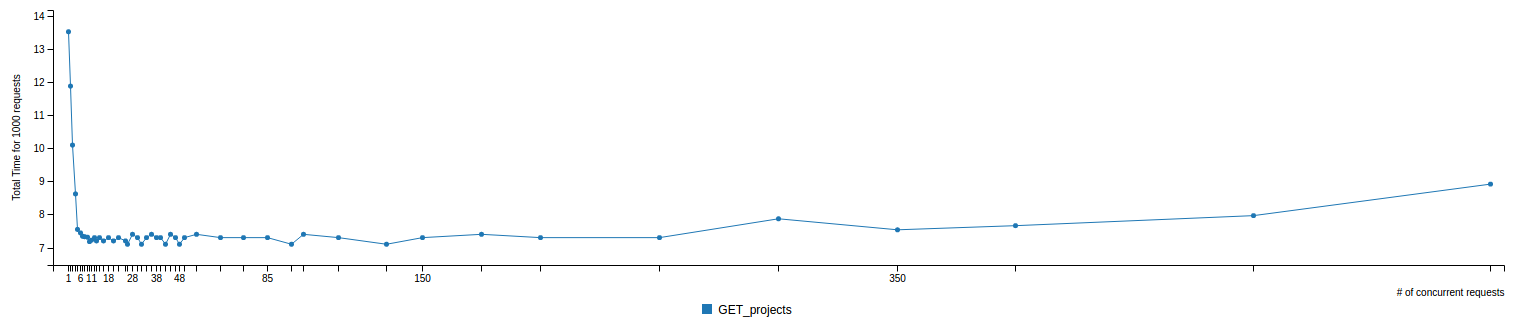
\includegraphics[width=1.2\linewidth]{post_projects.png}}
  \caption{POST projects route experiment}
\end{subfigure}
\begin{subfigure}{1\textwidth}
  \centering
  \centerline{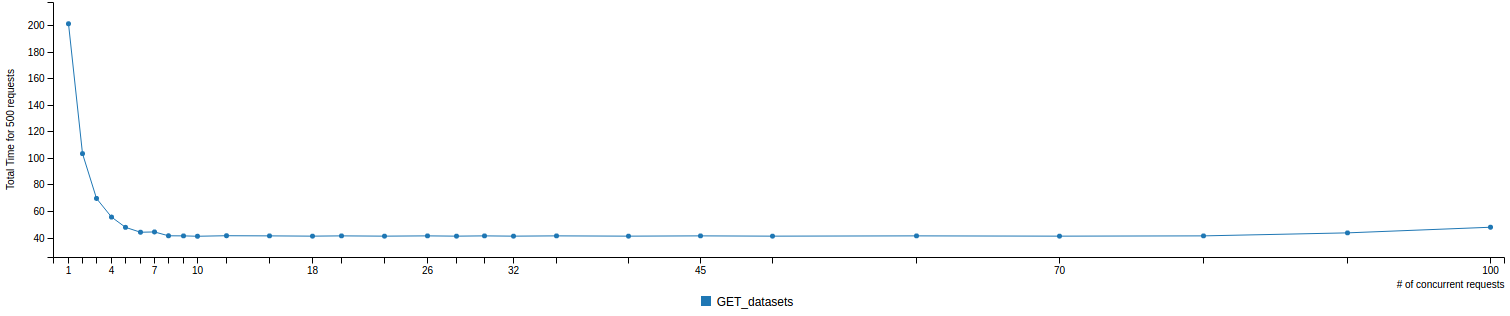
\includegraphics[width=1.2\linewidth]{get_datasets.png}}
  \caption{GET datasets route experiment}
\end{subfigure}
\begin{subfigure}{1\textwidth}
  \centering
  \centerline{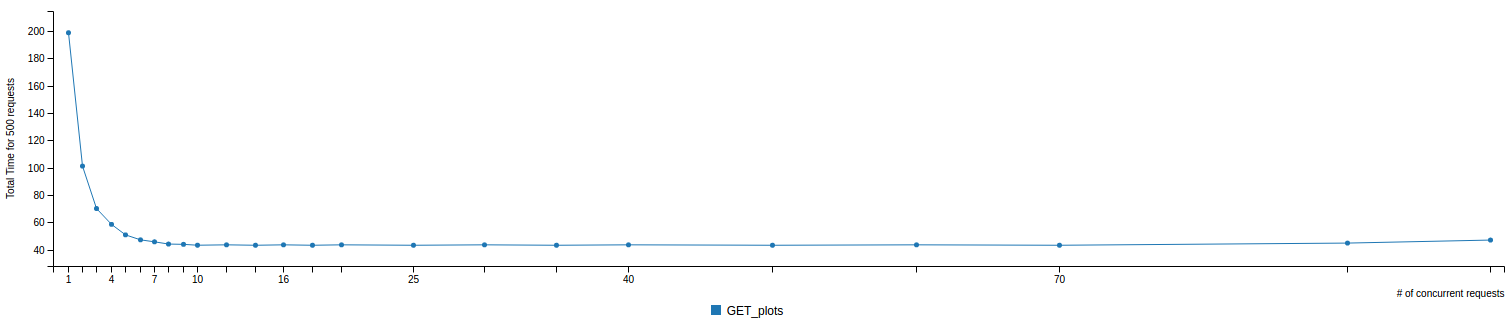
\includegraphics[width=1.2\linewidth]{get_plots.png}}
  \caption{GET plots route experiment}
\end{subfigure}
\caption{Total time for all requests / number of concurrent requests figure}
\label{experiment_fig}
\end{figure}


As we notice all the subfigures follow a specific pattern. Initially in all the subfigures the total time for the response of all the requests is considerably higher, compared to the following values of the diagrams. This is due to the low initial concurrency, which causes a delay until the requests are sent. That is, there is a lot of unused server-side processing power. In the case that "c=1", each request is sent after the completion of the previous sending, which explains the relatively high initial values. \par 
	Following, we observe in all the diagrams a stabilization of the total time of serving the requests, as the "c" increases. This is partially due to the adequate load the stress tool provides, so that there is no delay of the sending of the requests, but also because the server has enough time to respond without any delay. \par 
	At the end of the subfigures we notice that the total time for serving the requests starts to increase gradually. The reason is that the number of concurrent requests sent by the ab tool is now too high to be served by the server, and this is the cause of the delay. \par 
	We observe significant differences between the values of the diagrams, the most important being in the routes where python is used. To execute these routes, new child processes must be spawned. As the number of the concurrent requests increases, the spawned child processes oversaturate the function of the server. This is how the higher time values in serving the requests are explained.  

	
\section{Testing Timeout Errors in Concurrent Requests}
The basic characteristic of the second test scenario is the timeout value. A timeout occurs when the server fails to serve a request in a specific time period from the moment it was sent. In this test we set a relatively small timeout limit of two seconds and define each iteration in ten seconds per concurrency value. Gradually we raise the concurrency value and we calculate the number of served requests per second. The test scenario is finished when the first timeout error occurs. The results are presented in figure ~\ref{experiment_fig2}. \par 


\begin{figure}
\centering
\begin{subfigure}{1\textwidth}
  \centering
  \centerline{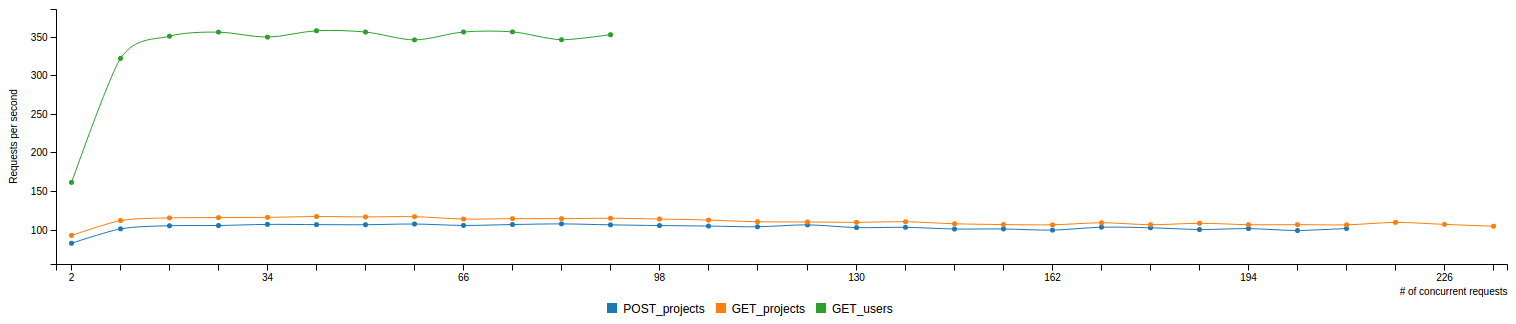
\includegraphics[width=1.2\linewidth]{error1.png}}
  \caption{Second experiment result}
\end{subfigure}
\begin{subfigure}{1\textwidth}
  \centering
  \centerline{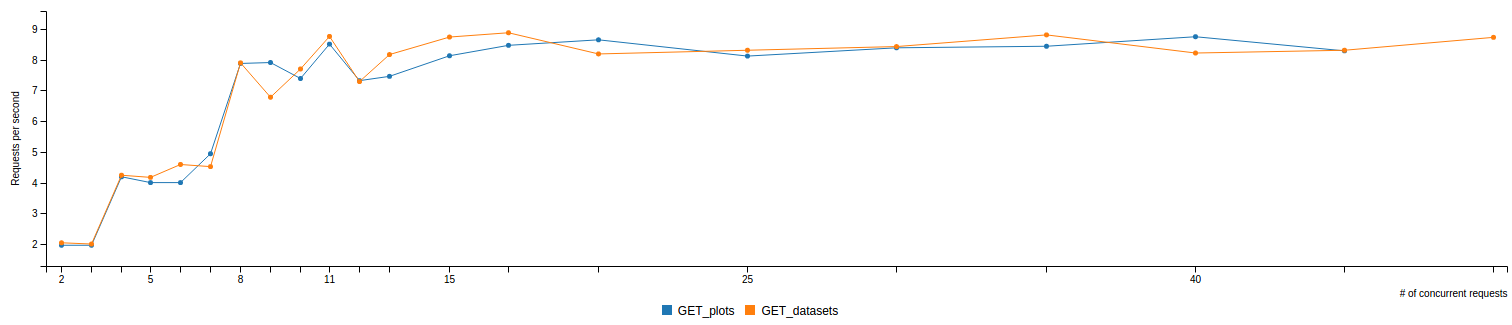
\includegraphics[width=1.2\linewidth]{error2.png}}
  \caption{Second experiment result}
\end{subfigure}
\caption{Requests per second / number of concurrent requests}
\label{experiment_fig2}
\end{figure}


We notice that the routes that use spawned python child processes serve far less requests per second, as expected. Additionally, these routes cause far sooner timeout errors. On the contrary, the rest of the routes serve many more requests per second and delay the occurence of timeout errors.








\chapter{Conclusions and Future Work}
\label{chapter7_cf}
\section{Conclusions}
In the scope of this diploma thesis we designed and implemented a back and front end framework globally developed in javascript, using the model driven software development approach. The framework provides entity to model mapping feautures, RESTful web service, data access object and CRUD operations for each model. The system utilizes a custom access control list module for user authorization. Also, the framework implements a method, which represents multidimentional hdf files in plots, in an efficient integrated way. The front-end tier of the framework utilizes the single page application design approach. \par 
	In order to present the framework not only as an idea, but also as an implemented concept, we designed and developed a demo application. The application's objective is the creation of user networks, in order to manipulate and visualize multidimentional datasets. Next we present the main advantages of our framework.

\paragraph{Extensibility} The framework follows the principles of model driven software development architecture, thus any extra operation can be added, either within the context of an already developed service, or as a new functionality with few lines of code. For example, an extra entity model or a route method may be easily added in the system.
	

\paragraph{No context switching} The framework is developed mainly in javascript. Therefore, the developer's productivity is increased, because only one programming language must be learned in order to evolve the current framework. Especially the front-end tier, was developed exclusively in pure javascript from scratch, without the usage of a large framework.


\section{Future Work}
The way in which the framework is designed and iplemented, offers us the potentiality of functionality extention in the future. Below we mention some possible extentions.

\paragraph{Server clustering}  A single instance of Node.js runs in a single thread. To take advantage of multi-core systems the user will sometimes want to launch a cluster of Node.js processes to handle the load. The node.js cluster module can be used to utilize this functionality, so the system scales on full load.

\paragraph{Mongodb replication and sharding} Sharding complications and replication fault tolerance will be studied in the future to optimize scalability.

\paragraph{Alternative methods in existing functionalities}
The framework functionality can be expanded in current operations. Upload file formats may be added (i.e csv files), in order to be converted and saved in the framework filesystem. Also, we can use different methods in plot sampling, such as mean values.
 
\paragraph{Image extraction for usage outside the system}
Right now is not possible the interaction between system users and none users. In the future extra features may be added to solve this problem, such as exporting plots in jpg format to share with users outside the application.

	 
 

%----------------------------------------------------------------------------------------
%	BIBLIOGRAPHY
%----------------------------------------------------------------------------------------

\printbibliography[heading=bibintoc]

%----------------------------------------------------------------------------------------

\end{document}  
